\chapter{Results}
\label{sec:4}
\section{Introduction}
\label{sec:4.1}  
The outline of this chapter is as follows: in \sectref{sec:4.2}, \sectref{sec:4.3} and \sectref{sec:4.4}, I will provide a description as well as an interpretation of the visualizations of the semantic field of \textit{beginnen}/inchoativity of SourceDutch, TransDutch\textsubscript{ENG} and TransDutch\textsubscript{FR} respectively, yielded on the basis of the methodological procedure developed in the previous chapter. Each description will consist of the following elements: (i) the results of the Hierarchical Agglomerative Cluster Analysis (carried out on the output of a Correspondence Analysis), (ii) a description of the prototype-based organization of the clusters in the dendrogram based on the distances of the centroids to the zero-point of the semantic space, (iii) a description of the prototype-based organization of the lexemes within each cluster based on the distances of the lexemes in each cluster to their cluster’s centroid, (iv) a description of the medoid of each cluster. The distances of the centroids to the zero-point of the semantic space (the prototypical center) inform us on the semasiological level about the prototype-based organization of the clusters (the meaning distinctions) in the semantic space (the semantic field of \textit{beginnen}). The distances of the lexemes to the centroid of the cluster give us more information on the onomasiological level about the prototype-based organization of the lexemes within each cluster. The medoid (the best exemplar) as well as the lexeme closest to the centroid of a cluster (the best representation of the abstract prototype) can be used to determine the most prototypical expression in each cluster. Finally, (v) an in-depth interpretation of each visualization representing a semantic field of \textit{beginnen}/inchoativity will be provided, on the basis of which a meta-label will be determined for each cluster so as to name the specific meaning distinction revealed by that cluster. The meta-labels that I will assign should be understood as a post-hoc, interpretative tool, applied to enhance my understanding of the rendered dendrograms. It should be clear that my attempt to present such a post-hoc interpretation of the quantitative and statistical information in terms of semantic change needs to be seen as a first exploration of the field of inchoativity and by no means an endpoint. In \sectref{sec:4.5}, \sectref{sec:4.6} and \sectref{sec:4.7} I will present my insights with respect to tendencies of levelling out, shining through and normalization each time on both the semasiological and the onomasiological level. The interpretations of the fields of SourceDutch, TransDutch\textsubscript{ENG} and TransDutch\textsubscript{FR} described in the previous sections will be used as a basis here. Statements about semasiological change will be based on the outcome of a statistical analysis and an interpretation of clusters as meaning distinctions. Conclusions about onomasiological change will be based on measurements of minimal (and hence subtle) differences in distances to an abstract prototype contained in the centroid. 

\section{SourceDutch}
\label{sec:4.2}  
\subsection{Results of the Hierarchical Agglomerative Cluster analysis}
\label{sec:4.2.1}  
Following the procedure described in \chapref{sec:3}, I carried out a HAC on the output of a CA. I first applied the statistical technique of CA. The scree plots in Figure~\ref{fig:4:50} shows the distribution of the variation over the latent dimensions of the CA. The cumulative scree plot (\figref{fig:4:51} right) shows that at least 5 dimensions are needed to represent more than 80\% of the variation.

\begin{figure}
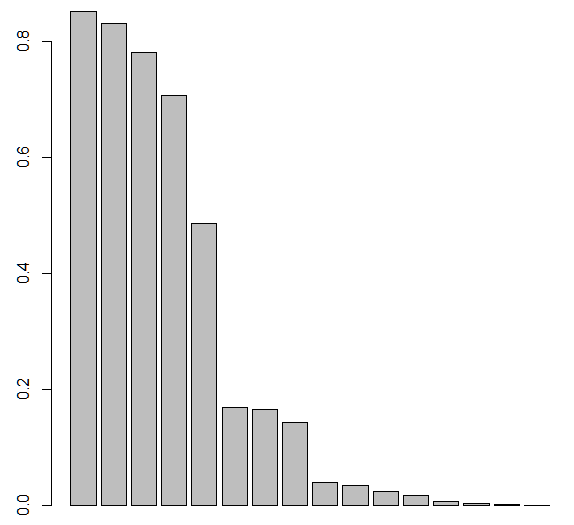
\includegraphics[width=.48\textwidth]{figures/Vandevoorde2-img50.png}\hfill%
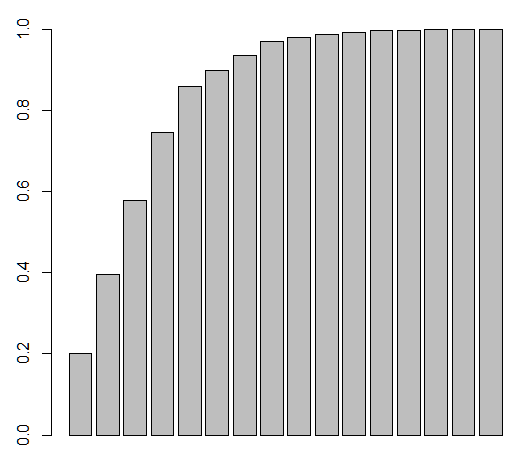
\includegraphics[width=.48\textwidth]{figures/Vandevoorde2-img51.png}
\caption{\label{fig:4:50}Left: Scree plot for SourceDutch. Right: \label{fig:4:51}Cumulative scree plot for SourceDutch}
\end{figure}

On the basis of the scree plot in \figref{fig:4:51} (right), I reduced the number of dimensions of the CA to 5. This step is important to avoid noisy (less informative) data patterns. A HAC was then carried out on the output of the CA. The cut-off point was set at a height of 4 (following the rationale described in \chapref{sec:3}),\footnote{Note that with \texttt{pvrect()}, which cuts off each cluster at the highest possible node with a significant $p$-value – the same cluster solution would have been obtained.} resulting in a cluster solution with 6 clusters: cluster n°1 contains \textit{oprichten} `to establish' and \textit{opzetten} `to set up'; cluster n°2 includes \textit{aanvang} `commencement', \textit{begin} `beginning' and \textit{start} `start'; cluster n°3 comprises \textit{opstarten} `to start up', \textit{starten} `to start', \textit{van} \textit{start} \textit{gaan} `to take off', \textit{beginnen} `to begin' and \textit{gaan} `to go'; cluster n°4 holds \textit{ontstaan} `to come into being' and \textit{openen} `to open'; cluster n°5 consists of \textit{komen} `to come', \textit{krijgen} `to get' and \textit{worden} `to become'; cluster n°6 contains \textit{eerst} `firstly'. I consider the result presented in \figref{fig:4:52} as a possible visualization of a semantic field of \textit{beginnen}/inchoativity in SourceDutch.

\begin{figure}  
% 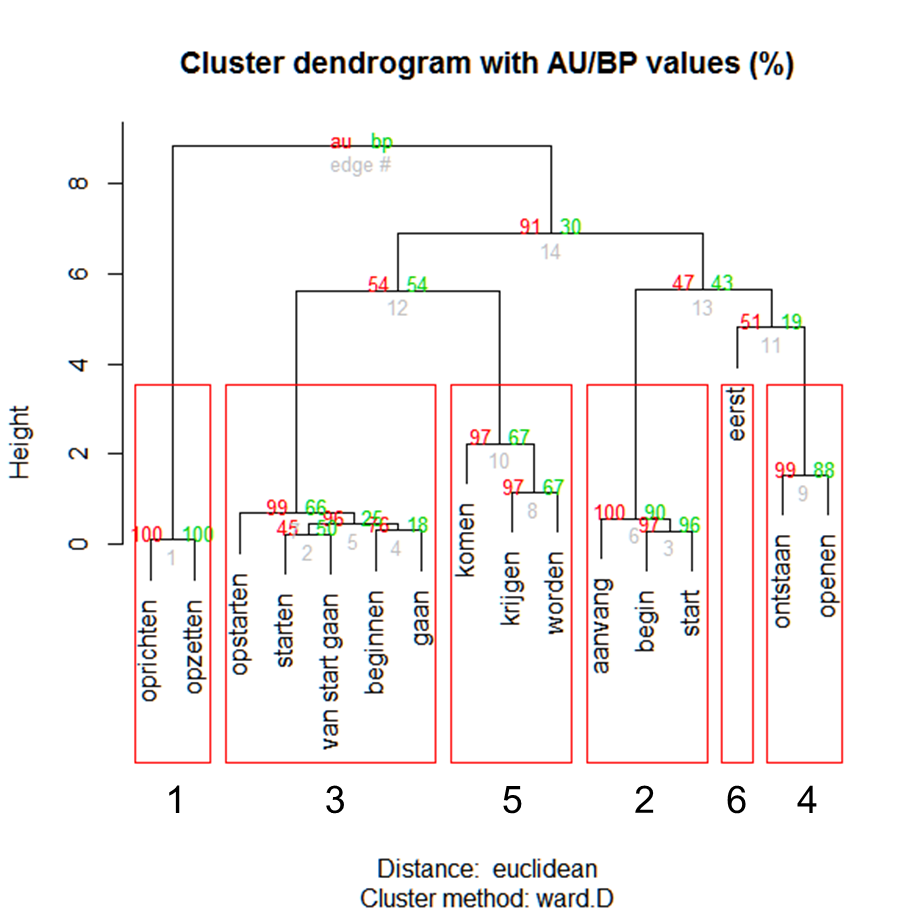
\includegraphics[height=.4\textheight]{figures/Vandevoorde2-img52.png}
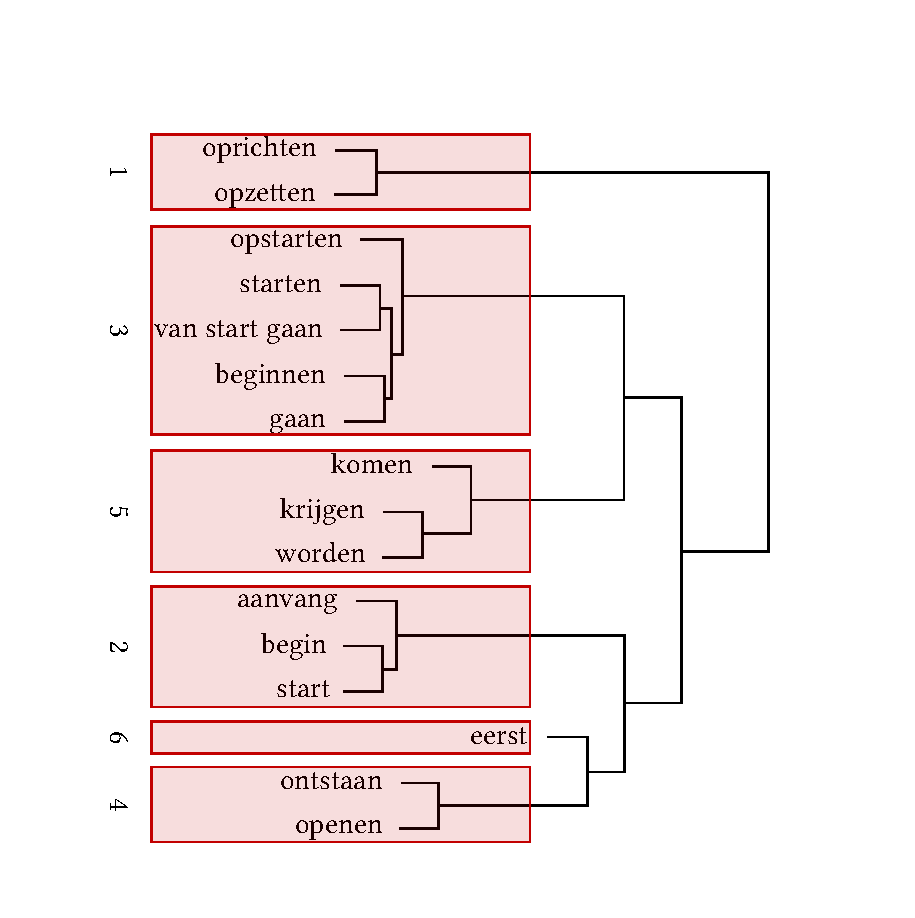
\includegraphics[width=.75\textwidth,trim=0 20 0 50]{figures/tree52.pdf}
\caption{\label{fig:4:52}  Dendrogram representing a semantic field of \textit{beginnen}/inchoativity for SourceDutch}
\end{figure}

In order to validate the chosen cluster solution with 6 clusters, I calculated the average silhouette width. I obtained an average silhouette width of 0.59 for this cluster solution, which is above the 0.50 threshold for good classification determined by Kaufman and Rousseeuw (see \sectref{sec:3.7.2.3}).

\begin{figure}
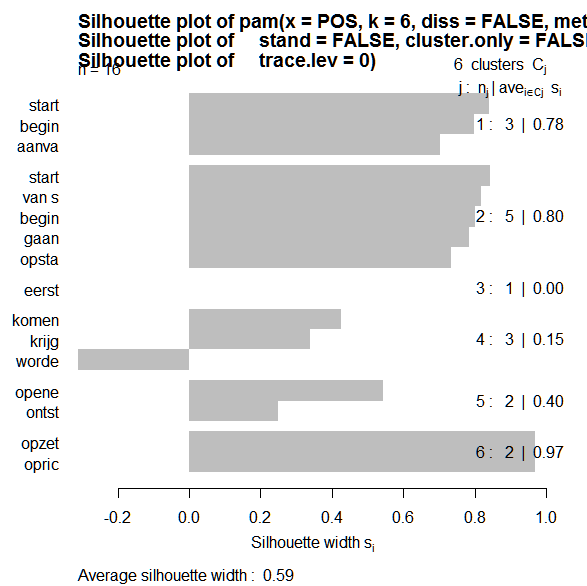
\includegraphics[height=.6\textwidth]{figures/Vandevoorde2-img53.png}
\caption{\label{fig:4:53}Average silhouette width for cluster solution with 6 clusters for SourceDutch}
\end{figure}

A $k$-means clustering was carried out as a second validation technique for the chosen cluster solution. When a cluster solution with 6 clusters was requested, the $k$-means clustering shown in \figref{fig:4:54} was proposed (the numeral below each lexeme assigns it to a specific cluster).
  
\begin{figure}
% 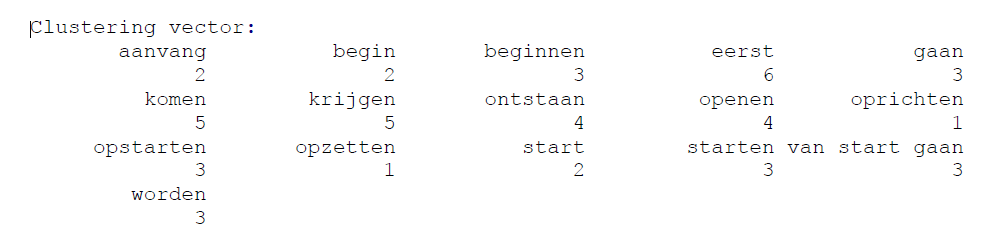
\includegraphics[width=\textwidth]{figures/Vandevoorde2-img54.png}
% \footnotesize
\centering%
\begin{lstlisting}
Clustering vector:
      aanvang       begin    beginnen      eerst             gaan 
            2           2           3          6                3         
        komen     krijgen    ontstaan     openen        oprichten         
            5           5           4          4                1         
    opstarten    opzetten       start    starten   van start gaan         
            3           1           2          3                3         
       worden                                            
            3                                      
\end{lstlisting}     
\caption{\label{fig:4:54}$k$-means clustering with 6 clusters for SourceDutch}
\end{figure}

Note that the only difference with the output of the HAC is that \textit{worden} is assigned to the cluster containing \textit{starten}, \textit{van} \textit{start} \textit{gaan,} \textit{opstarten,} \textit{beginnen}, and \textit{gaan}. On the basis of both validation techniques, I consider my cluster solution for SourceDutch as a good classification. In addition, as a result of the $k$-means clustering it can be concluded that the clustering of the polyfunctional verb \textit{worden} seems to be uncertain.

\subsection{Prototype-based organization of the clusters in the dendrogram (semasiological level)}
\label{sec:4.2.2}  
In order to obtain more information about the prototype-based organization of the clusters (meaning distinctions) within each dendrogram, I determined the distance of the centroids of each cluster to the origin or zero-point of the semantic space (the prototypical center). The centroids were subsequently mapped onto a dot chart (\figref{fig:4:55}). The cluster closest to the zero-point is considered to be the most central one in the semantic space.

\begin{figure} 
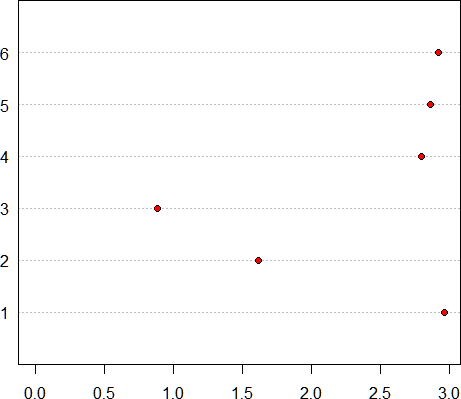
\includegraphics[height=.4\textheight]{figures/Vandevoorde2-img55.png}\vspace*{\baselineskip}
\scriptsize
\begin{tabular}{l>{\itshape}l}
\lsptoprule
Cluster 6 & eerst\\
Cluster 5 & krijgen{\normalfont,} komen{\normalfont,} worden\\
Cluster 4 & ontstaan{\normalfont,} openen\\
Cluster 3 & Starten{\normalfont,} van start gaan{\normalfont,} opstarten{\normalfont,} beginnen{\normalfont,} gaan\\
Cluster 2 & aanvang{\normalfont,} begin{\normalfont,} start\\
Cluster 1 & opzetten{\normalfont,} oprichten\\
\lspbottomrule
\end{tabular}
\normalsize
\caption{\label{fig:4:55}Dot chart presenting the distance of the cluster centroids to the zero-point of the semantic space of SourceDutch}
\end{figure}

Note that the numerals on the y-axis of the dot chart in \figref{fig:4:55} were assigned by a previously established list (based on the output of the cluster analysis), necessary to calculate the cluster centroids (the order of the assigned numerals is arbitrary). The content of each cluster number is resumed in the table accompanying \figref{fig:4:55}. The dot chart shows us that cluster n°3, containing \textit{starten}, \textit{van} \textit{start} \textit{gaan}, \textit{opstarten}, \textit{beginnen} and \textit{gaan} is the most central cluster in the analysis, rather closely followed by cluster n°2 comprising \textit{aanvang,} \textit{begin} and \textit{start}. Then, clusters n°4 (\textit{ontstaan} and \textit{openen}), n°5 (\textit{komen}, \textit{krijgen} and \textit{worden}), n°6 (\textit{eerst}) and n°1 (\textit{oprichten,} \textit{opzetten)} are situated considerably further away but at an almost equal distance of the plot’s origin.

\subsection{Prototype-based organization of the lexemes within each cluster (onomasiological level)}
\label{sec:4.2.3}  
Next, the prototype-based organization of the lexemes within each cluster was inspected by measuring the distance of the lexemes of each cluster to the centroid of the cluster they belong to. In addition, I calculated the medoid of each cluster. Both the lexeme closest to the centroid and the medoid can be used to determine which lexical item in each cluster can be considered as the most prototypical expression of that cluster although I regard the two measures as different views on prototypes: the lexeme closest to the centroid is considered as the best possible representation of the abstract prototype contained in the centroid, the medoid indicates the best example as the prototype of the cluster it belongs to.

\subsubsection{Centroids}
\label{sec:4.2.3.1}  
Each of the six dot charts (Figures~\ref{fig:4:56}--\ref{fig:4:61}) represents one of the six clusters of SourceDutch. The centroid of the represented cluster is taken as the zero-point of the dot chart, so that the lexemes pertaining to this cluster are the closest ones to the zero-point of the dot chart. This allows me to visualize which lexemes are more central, and which ones more peripheral in the cluster. In addition, these visualizations also show the distance of the lexemes of all the other clusters to the represented cluster centroid. This is especially interesting for lexemes of which the proposed clustering on the basis of the HAC appeared uncertain (e.g. \textit{worden}).

\begin{figure}
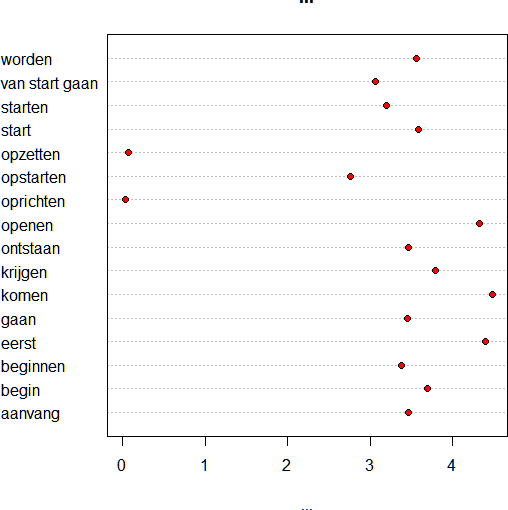
\includegraphics[width=.48\textwidth,trim=0 15 0 25]{figures/Vandevoorde2-img56.png}\hfill%
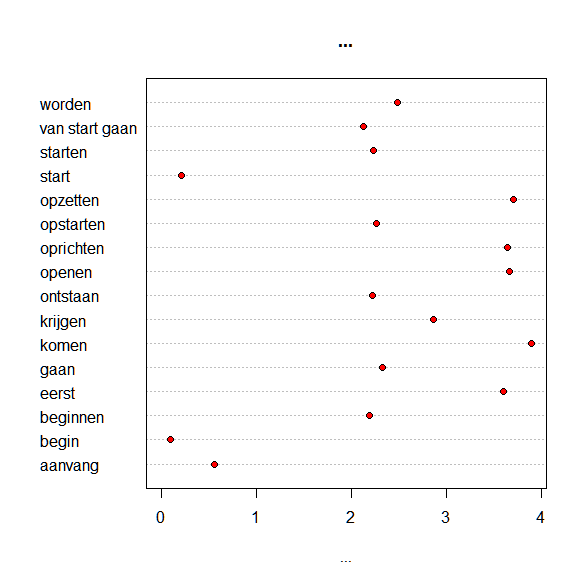
\includegraphics[width=.48\textwidth,trim=0 15 0 25]{figures/Vandevoorde2-img57.png}
\caption{\label{fig:4:56}Cluster n°1 (left) and n°2 (right) for SourceDutch.\label{fig:4:57}}
\end{figure}

\begin{figure}
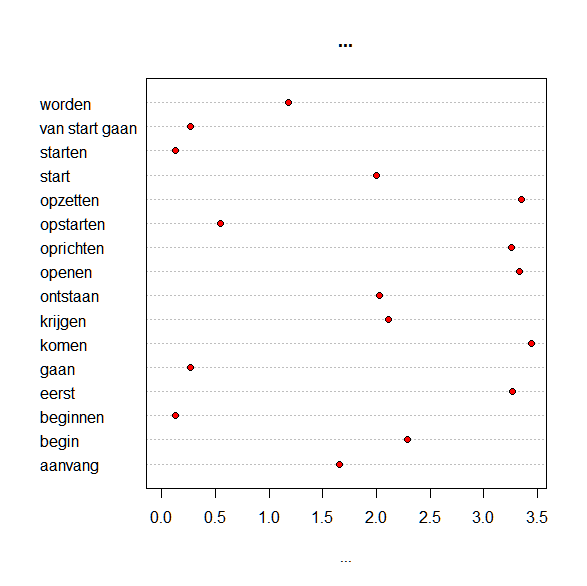
\includegraphics[width=.48\textwidth,trim=0 15 0 25]{figures/Vandevoorde2-img58.png}\hfill%
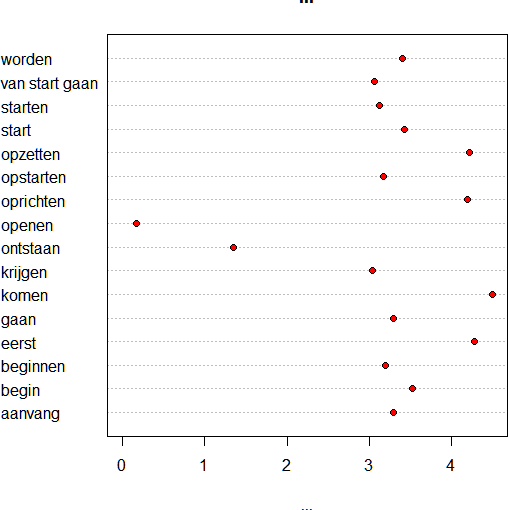
\includegraphics[width=.48\textwidth,trim=0 15 0 25]{figures/Vandevoorde2-img59.png}
\caption{\label{fig:4:58}Cluster n°3 (left) and n°4 (right) for SourceDutch.\label{fig:4:59}}
\end{figure}

\begin{figure}
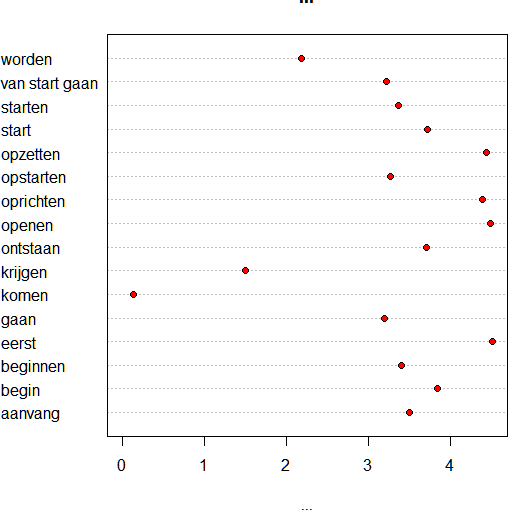
\includegraphics[width=.48\textwidth,trim=0 15 0 25]{figures/Vandevoorde2-img60.png}\hfill%
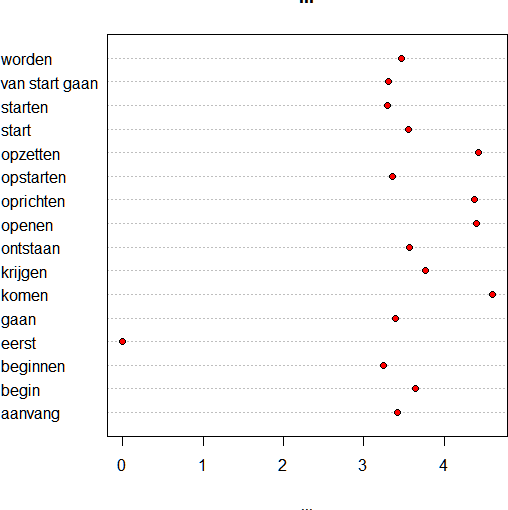
\includegraphics[width=.48\textwidth,trim=0 15 0 25]{figures/Vandevoorde2-img61.png}
\caption{\label{fig:4:60}Cluster n°5 (left) and n°6 (right) for SourceDutch.\label{fig:4:61}}
\end{figure}


Since the difference in distance of the members of a same cluster to their cluster’s centroid is often minimal, I used the calculated distances (which are represented by the dots in the dot charts) to evaluate the distances to the centroids (see \tabref{appendix-table-H}, Appendix~\ref{ch:C}).

For cluster n°1, the distance from \textit{opzetten} to the centroid is 0.06749455, whereas the distance from \textit{oprichten} to the centroid is 0.02952887, implying that \textit{oprichten} is closer to the centroid, and can thus be considered as the best representation of the abstract prototype of cluster n°1. For cluster n°2, the distance from \textit{start} to the centroid is 0.20740218 and the distance from \textit{begin} to the centroid is 0.08908994. This shows that \textit{begin} is closer to the centroid and can be considered as the best representation of the abstract prototype of cluster n°2. For cluster n°3, four lexemes are very close to the zero point. \textit{Van} \textit{start} \textit{gaan,} \textit{gaan} and \textit{opstarten} are slightly further away from the cluster’s centroid, but the difference in distance between \textit{starten} and \textit{beginnen} is minimal. The distance from \textit{starten} to the centroid is 0.1264550, and the distance from \textit{beginnen} to the centroid is 0.1254173. Hence, \textit{beginnen} is indicated as the cluster’s best representation of the abstraction of the prototype. With regard to cluster n°4, \figref{fig:4:59} (right) clearly shows that \textit{openen} is the closest lexeme to the centroid, and can hence be considered as the best representation of the abstract prototype of this cluster. As for cluster n°5, \textit{komen} can clearly be distinguished as the closest lexeme to the centroid, and is indicated as its best representation of the abstract prototype. Finally, it is unnecessary to indicate the best representation of the abstract prototype for cluster n°6, which is a singleton cluster with \textit{eerst}.

\subsubsection{Medoids}
\label{sec:4.2.3.2}  
A second quantitative possibility to obtain more information about the organization of the lexemes within each cluster is to calculate its medoid. The medoid assigns one object in the cluster from which the average distance to all other objects is the smallest \citep[164]{divjak_structuring_2010}. The medoids for the clusters are summarized in \tabref{tab:4:14} and compared to the lexeme closest to the centroid as determined above. The table shows that the medoid and the lexeme closest to the centroid never converge (clusters n°1, 4 and 6 are disregarded since they have only one or two members):

\begin{table}
\caption{\label{tab:4:14}Comparison of medoids and lexemes closest to the centroids for SourceDutch}
\begin{tabularx}{\textwidth}{XXl} 
\lsptoprule
Cluster & Medoid & Lexeme closest to centroids\\
\midrule
Cluster n°2 & \itshape Start   & \itshape Begin\\
Cluster n°3 & \itshape Starten & \itshape Beginnen\\
Cluster n°5 & \itshape Krijgen & \itshape Komen\\
\lspbottomrule
\end{tabularx}
\end{table}

The divergence between the closest lexeme to the centroid and the medoid of a cluster for all clusters increases the uncertainty about which lexeme can be considered as the most central one. In addition, the difference in distance to the centroid is minimal for some clusters, especially for cluster n°3 (\textit{beginnen} vs.\ \textit{starten}) and cluster n°2 (\textit{begin} vs.\ \textit{start}). It is noteworthy that for those two clusters with a minimal difference in distance to the centroid, it is the second closest lexeme that is indicated as the medoid each time. This is potentially very interesting and could indicate a field of tension between several of the more central expressions in each cluster.

The diverging evidence from medoids and distance to centroids makes it difficult to put forward the outcome of the one or the other measure as the better one to determine the most prototypical expression for each cluster, all the more because they have been linked to different views on prototype. As a consequence, neither the lexeme closest to the centroid nor the medoid will be used as a meta-label to name the specific meaning distinction of the cluster.

\subsection{Interpretation of the semantic field of \textit{beginnen}\slash inchoativity for SourceDutch}
\label{sec:4.2.4}  
I will now provide an interpretation of the visualization representing a semantic field of \textit{beginnen}/inchoativity for SourceDutch.\footnote{Substantial parts of the interpretations of the visualizations of SourceDutch, TransDutch\textsubscript{ENG} and TransDutch\textsubscript{FR} in \sectref{sec:4.2.4} \sectref{sec:4.3.4} and \sectref{sec:4.4.4} of this book have been first presented in \citep{VandevoordeEtAl2017}, an article which is under copyright. Its publisher should be contacted for permission to re-use or reprint the material in any form.} This interpretation will be used to determine a meta-label for each cluster so as to name the specific meaning distinction revealed by that cluster. The meta-labels that I will assign should be understood as a post-hoc, interpretative tool, applied to enhance my understanding of the rendered dendrograms. Note that I do not consider the meta-labels as a validation of the discerned cluster organization – if this had been my intention, I should have determined the labels beforehand. As determined in \sectref{sec:3.8.1.4}, information from three types of sources will be used (in addition to the information about the prototype-based organization of the clusters in the field and the lexemes in each cluster): (i) corpus examples from the DPC containing the lexemes which make up a cluster (ii) attestations in reference works and (iii) information from the lexical database Cornetto \citep{vossen_cornetto_2008, spyns_cornetto:_2013}. 

I consider cluster n°3 as the most central cluster or \textsc{reference cluster}, representing the idea of \textsc{general onset}. There are two arguments to justify this. First, on the semasiological level this cluster’s centroid is the closest one to the origin of the semantic space and hence, the most central one in the prototype-based organization of the semantic field. Second, on the onomasiological level, Figures~\ref{fig:4:56}--\ref{fig:4:61} – which depict the distances of the lexemes to each of the centroids of the other clusters – show that the lexemes of cluster n°3 are always situated at a fairly equal distance of the centroids of all the other clusters (somewhat in the middle of each plot). This implies that cluster n°3 shows the least deviation with respect to the other clusters (the lexemes of cluster n°3 are all equally similar to the abstract prototype of each of the other clusters). Third, cluster n°3 holds the initial lexeme \textit{beginnen}, which was selected to initiate the SMM++ retrieval task since it is considered as the most prototypical expression of inchoativity (based on corpus frequency and etymological age). The cluster containing \textit{beginnen} is believed to hold the most prototypical expressions of inchoativity.

Cluster n°3 contains three different sub-nodes, one with \textit{opstarten} `to start up', and two other, interrelated sub-nodes; one with \textit{starten} `to start' and \textit{van} \textit{start} \textit{gaan} `to take off' and another one with \textit{beginnen} `to begin' and \textit{gaan} `to go'. In my opinion, these latter two interrelated sub-nodes indicate an additional meaning-distinction within the meaning-distinction indicated by cluster n°3. Besides \textit{beginnen}, \textit{starten} is also a typical expression of inchoativity, and the two are often considered as near-synonyms \citep[223]{schmid_introspection_1996}. \citet{lewandowska-tomasczyk_corpus-based_2009} – based on research by \citet{biber_longman_1999} and \citet{schmid_cottage_1993}, following \citet{quirk_comprehensive_1985} – conclude the following for the English phasal verbs \textit{to} \textit{start} and \textit{to} \textit{begin}:

\begin{quote}
\textbf{Begin} then gives a view into the state after onset of the action: it expresses modality\slash intentionality and refers to \textbf{later} \textbf{states} \textbf{of} \textbf{affairs}. It typically applies to cognitive-emotive events and non-perceivable things. \textbf{Start}, on the other hand, focuses on the \textbf{actual} \textbf{action}, the actual beginning, the very moment of transition from non-action to action. It is dynamic and applies to visible change and actions (\citealt[279]{lewandowska-tomasczyk_corpus-based_2009}, my emphasis).
\end{quote}

The subdivision observed in the (Dutch) results into verbs formally related to \textit{starten} `to start' such as \textit{van start gaan} `to take off' on the one hand (hence: \textsc{action} verbs), and verbs formally related to \textit{beginnen} `to begin' (hence: \textsc{state after onset} verbs) on the other hand, corroborates the distinction made by Divjak \& Gries. The attested distinction between \textit{to start} and \textit{to begin} seems to hold for Dutch \textit{starten} and \textit{beginnen}, too. Recall that the two lexemes closest to the centroid of this cluster are indeed \textit{beginnen} (0.1254173) and \textit{starten} (0.1264550); the minimal difference in distance to the centroid between these two lexemes further shows that there is some kind of ``competition'' going on between the two and that either of the two would be a good candidate to be the best representation of the abstract concept of the prototype. Further note that the distinction between \textsc{action} and \textsc{state after onset} is not indicated in Cornetto, which classifies all the lexemes of cluster n°3 as the same semantic type, i.e. \textsc{action} (“verb that describes an action that is usually controlled by the subject of the verb”), with the only exception that \textit{beginnen} can also be granted the semantic type \textsc{process} (“a dynamic event that is not initiated by an actor capable of acting with volition”). According to the lexical-semantic database Cornetto \citep{vossen_cornetto_2008}, \textit{gaan} `to go',\footnote{Recall that observations of \textit{gaan} in the construction \textit{van start gaan} are not included here.} which somewhat oddly seems to be clustered with \textit{beginnen}, is defined as “beginnen iets te doen” -- `to begin to do something', and \textit{beginnen} as “iets gaan doen” -- `to go and do something'. The definitional relation indicated by Cornetto seems to underpin the semantic relationship indicated by the clustering of \textit{beginnen} and \textit{gaan}. In addition, according to the Algemene Nederlandse Spraakkunst (General Dutch Grammar) \citep{haeseryn_algemene_2012}, the first of two subtypes of \textit{gaan} “without the meaning of motion” is the subtype where \textit{gaan} has the meaning of “‘(geleidelijk) overgaan tot’, ‘beginnen te’ (inchoatief aspect)” -- `(gradually) move on to, to begin to (inchoative aspect)'. The relatedness between \textit{starten} and \textit{beginnen} is also further substantiated by the definitions of \textit{starten} in Cornetto: 

\begin{enumerate}[label=(\roman*)]
\item “beginnen van iets (niet-causatief)” -- `beginning of something (non-cau\-sa\-tive)'
\item “doen beginnen (causatief)” -- `to make begin (causative)'
\item “(van apparaten) beginnen te functioneren” -- `(of devices) begin to function', 
\end{enumerate}
which all bear \textit{beginnen} in their Dutch definition. The label of \textsc{reference cluster}\slash \textsc{general onset} is assigned to cluster n°3, with \textsc{reference cluster} referring to the cluster’s position in the cluster hierarchy and \textsc{general onset} representing the overall semantic content of this cluster. An additional meaning distinction is furthermore discerned within this cluster between \textsc{action} verbs (to which I will assign the label \textsc{action}) and \textsc{state after onset} verbs (which will be labeled as \textsc{state after onset}).

Cluster n°2 contains \textit{begin} and \textit{start} – which are the nominal derivatives of the prototypical verbs \textit{beginnen} and \textit{starten} -- as well as \textit{aanvang.} On the semasiological level, the centroid of this cluster is the second closest one to the zero-point, implying its relative centrality in the semantic space. The centroid of cluster n°2 is also fairly close to the centroid of the \textsc{reference cluster}, which seems to confirm the close relationship between the two clusters. The third lexeme in this cluster, \textit{aanvang} is again a noun, but differs from \textit{begin} and \textit{start} in that it belongs to a more formal register \citep{van_dale_van_2015}. Although the majority of the lexemes in the dendrogram are verbs, there are indeed three nouns represented, which are now grouped together into one cluster. A possible explanation for the separate clustering of the nouns and verbs in this analysis goes as follows: a nominal derivative such as \textit{begin} and its ``root'' verb \textit{beginnen} appear in different syntactic contexts but are likely to appear in similar lexical environments. Since this analysis can be considered as a translational analysis, which uses translation to lay bare meaning, it seems plausible that the syntactic environment of a sentence is more likely to primarily impose choice of word class (but not word choice -- e.g. a noun is more likely to be translated by a noun, and a verb by a verb), which could explain why the translational method favors a word-class dependent clustering of lexemes. Based on the previous reflection, the meta-label \textsc{general onset} (\textsc{noun}) is chosen for cluster n°2. \textsc{general onset} indicates that this cluster situates itself close to the \textsc{reference cluster} of \textsc{general onset}; the addition of (\textsc{noun}) refers to the word-class dependence of this cluster.

Cluster n°1 holds the verbs \textit{oprichten} `to set up, to establish' and \textit{opzetten} `to set up'. Within Cornetto, \textit{oprichten} is defined as \textit{opzetten}. I consequently consider them as near-synonyms. In Cornetto, \textit{oprichten} is associated with the setting up of an association, a party, a school, whereas \textit{opzetten} is associated with the setting up of a project, an activity, a bank, a company, a business. Corpus examples (\ref{ex:10} and~\ref{ex:11}) from the DPC show that \textit{oprichten} can, like \textit{opzetten}, be used in business-like contexts:

\ea (dpc-arc-002048-en)\label{ex:10}\\
In 2000 \Highlight{zetten} de twee bedrijven een joint venture \Highlight{op} in Turkije. Vandaag doen zij dat opnieuw in Roemenië.\smallskip\\\relax
\textsc{source}: `In 2000, the two companies \Highlight{set up} a joint venture together in Turkey and today they are launching another in Romania.'
\ex (dpc-bco-002345-en, all emphases are mine)\label{ex:11}\\
Company1 versterkt zijn positie in het Oosten en \Highlight{richt} filialen \Highlight{op} in Australië en Taiwan\smallskip\\\relax
\textsc{source}: `Company1 strengthens its position in the east and \Highlight{starts up} subsidiaries in Australia and Taiwan.'
\z

On the onomasiological level, the difference in distance of the two lexemes to their cluster’s centroid was very small. Although \textit{oprichten} (0.02952887) was situated slightly closer to the centroid, \textit{opzetten} (0.06749455) was indicated as the medoid. This information further substantiates the idea that \textit{oprichten} and \textit{opzetten} are indeed near-synonyms. What seems to distinguish this cluster from the cluster of \textsc{general onset} is that \textit{opzetten} and \textit{oprichten} appear to indicate a specific type of action, related to the setting up of a project, a business, a company, etc. I will therefore add the label \textsc{specific action} to cluster n°1.

The lexemes \textit{komen} `to come', \textit{krijgen} `to get', \textit{worden} `to become' in cluster n°5 share the semantic characteristic that their inchoative aspect is non-lexicalized. By this I mean that these verbs’ potential to express inchoativity is not directly apparent from the verbs themselves, but that these verbs receive their inchoative value from the context they are used in (compared to, for instance, \textit{beginnen}, in which the inchoative aspect is lexicalized, and hence, directly apparent irrespective of the context it is used in) as the following example shows (note that, in this example \REF{ex:12}, the inchoative aspect is explicitated by its translation):

\ea\label{ex:12}(dpc-arc-002053-nl, my emphasis)\\
`SteelUser is er \Highlight{gekomen} om onze klanten het leven een stuk aangenamer en eenvoudiger te maken, […].'\smallskip\\\relax
\textsc{target}: `SteelUser was \Highlight{set up} to make life simpler and more comfortable for our clients, [...].'
\z

In Cornetto, the inchoative aspect of the three verbs is implicitly present in one of the definitions of \textit{komen}, viz., \textit{beginnen te spreken} `start to speak', of \textit{krijgen}, viz., \textit{in een situatie terechtkomen} `to find oneself in a situation', and in the examples provided by Cornetto for the copulative verb \textit{worden} `to become', \textit{boos\slash ziek\slash misselijk worden} `to become angry\slash ill\slash nauseated'. The meta-label chosen for this cluster is \textsc{non-lexicalized inchoativity}.

\textit{Ontstaan} `to come into being' and \textit{openen} `to open' make up cluster n°4. \textit{Ontstaan} is defined as \textit{tot stand komen} `to come about' in Cornetto. \textit{Openen}, in its inchoative meaning, is defined as (i) \textit{laten beginnen} `to let begin' when its semantic type is action (\textit{describing an action usually controlled by the subject of the verb}) and as (ii) \textit{opengaan} `to open' when its semantic type is process (\textit{not initiated by an actor capable of acting with volition}). The examples in Cornetto indicate that \textit{ontstaan} is often used to indicate the coming into being of abstract processes such as fights or quarrels (\textit{ruzie\slash onenigheid ontstaat} `a fight\slash a disagreement arises'), or for the coming into being of natural phenomena such as mountains or rivers (\textit{een gebergte ontstaat} `a mountain chain comes into being'; \textit{een rivier ontstaat uit een bron} `a river originates from a source'). \textit{Openen} is used to introduce the beginning of an event, either as an action (controlled by the subject of the verb), as in \textit{een symposium openen} `to open a symposium' or as a process (not initiated by an actor capable of acting with volition), as in \textit{het symposium opent} `the symposium begins'. Although this is not explicitly mentioned in Cornetto, the corpus furthermore (example \ref{ex:13}) shows that \textit{openen} can, just as \textit{ontstaan} refer to abstract processes, such as the coming into being of a right:

\ea\label{ex:13}(dpc-fsz-001052-nl, my emphasis)\\
Ik kan het recht openen op een tegemoetkoming omdat ik tot 21 jaar de verhoogde kinderbijslag genoot.
\glt `I can open the right on subsidy because I received increased family allowance until the age of 21.'
\z

The particularity of \textit{openen} in this field is that its inchoative meaning is in fact a metaphorical meaning extension of its clear literal meaning (`to open a door, a window'). `To open a new business unit' indicates that a new business unit is set up\slash comes into being, as illustrated in example \REF{ex:14} below:

\ea\label{ex:14}(dpc-lan-001674-nl, my emphasis)\\
In het kader van de concentrische groei,[…], opende men een Nederlandse distributieafdeling in Tilburg.\\\relax
\textsc{target:} `Within the framework of concentric growth, [...], a Dutch distribution department was set up in Tilburg.'
\z

The meaning distinction of the clustering of \textit{openen} and \textit{ontstaan} will tentatively be captured with the meta-label \textsc{onset of abstract processes}, which seems to be the common denominator of the two verbs.

Finally, cluster n°6 is a singleton cluster containing the adverb \textit{eerst} `firstly', which presents a clear inchoative meaning. Again, just as nouns were not clustering with verbs, the only adverb in the set of candidate lexemes does not cluster with any other lexemes, further substantiating the previously made observation that the method favors word-class dependent clustering.

In sum, I labeled the different meaning distinctions (clusters) within the semantic field of \textit{beginnen}/inchoativity as follows (see \figref{fig:4:61b}): cluster n°3 (\textit{opstarten} `to start up', \textit{starten} `to start', \textit{van start gaan} `to take off', \textit{beginnen} `to begin' and \textit{gaan} `to go') is labeled as \textsc{reference cluster}\textit{/}\textsc{general onset}. Within cluster n°3, I have furthermore discerned an additional meaning distinction between \textit{beginnen} `to begin', \textit{gaan} `to go' labeled as \textsc{state after onset} and \textit{starten} `to start', \textit{van start gaan} `to take off' labeled as \textsc{action}. Cluster n°2 (\textit{aanvang} `commencement', \textit{begin} `beginning' and \textit{start} `start') is labeled as \textsc{general onset} (\textsc{noun}), cluster n°1 (\textit{oprichten} `to establish' and \textit{opzetten} `to set up') received the label {\textsc{specific}} \textsc{action}, cluster n°5 (\textit{komen} `to come', \textit{krijgen} `to get' and \textit{worden} `to become') is labeled as {\textsc{non-lexicalized inchoativity}}. Cluster n°4 (\textit{ontstaan} `to come into being' and \textit{openen} `to open') is labeled as {\textsc{onset of abstract processes}}. These meta-labels are far from ideal descriptions of the clusters and are naturally open for discussion. As explained in \sectref{sec:4.3.4}, the meta-labels merely serve to enhance my understanding of the clusters and to facilitate the further description of what happens to the meaning distinctions revealed by the clusters in the different semantic fields.

\begin{figure}
% 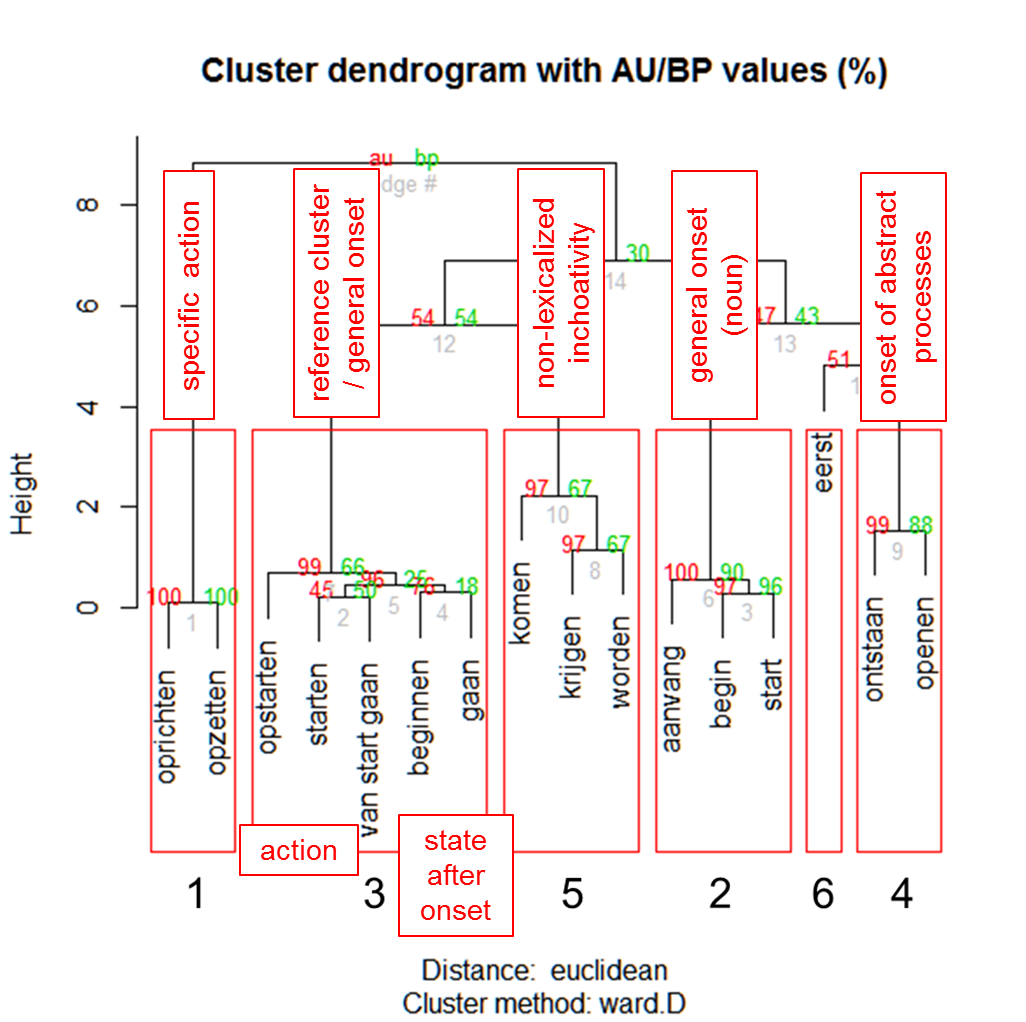
\includegraphics[height=.4\textheight]{figures/Vandevoorde2-img62.png}
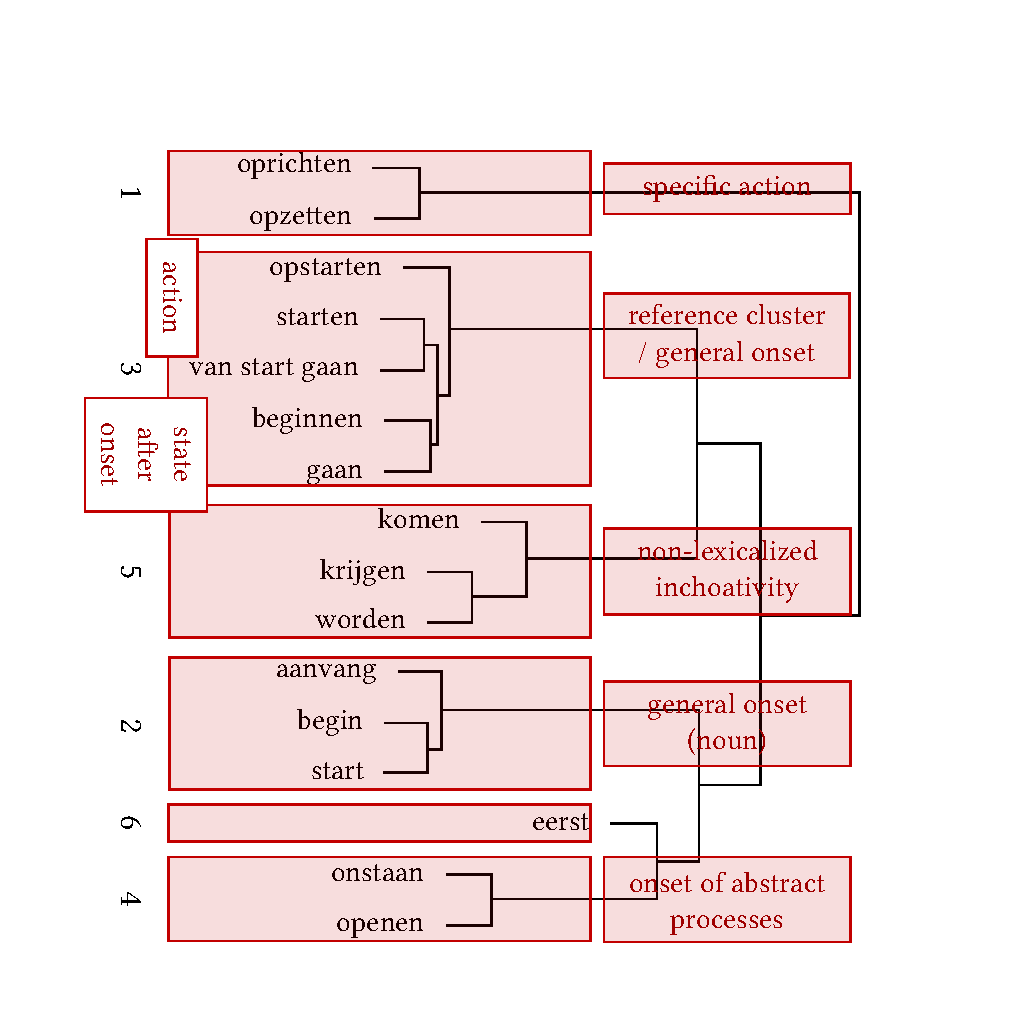
\includegraphics[width=\textwidth]{figures/tree62.pdf}
\caption{\label{fig:4:61b}Dendrogram representing a semantic field of \textit{beginnen}/inchoativity for SourceDutch with meta-labels}
\end{figure}

\section{TransDutch\textsubscript{ENG}}
\label{sec:4.3}  
For the description and interpretation of TransDutch\textsubscript{ENG}, I repeated the steps carried out for SourceDutch presented in the previous section.

\subsection{Results of the Hierarchical Agglomerative Cluster analysis}
\label{sec:4.3.1}  
The distribution of the variation over the latent dimensions of the CA is shown in \figref{fig:4:62}. The number of dimensions of the CA is reduced to 4.\footnote{Although 3 dimensions seemed to suffice here to represent more than 80\% of the variation, I opted for 4 dimensions, which is the minimum number of dimensions required to carry out \texttt{pvclust()} in the next step of this analysis.}


\begin{figure}
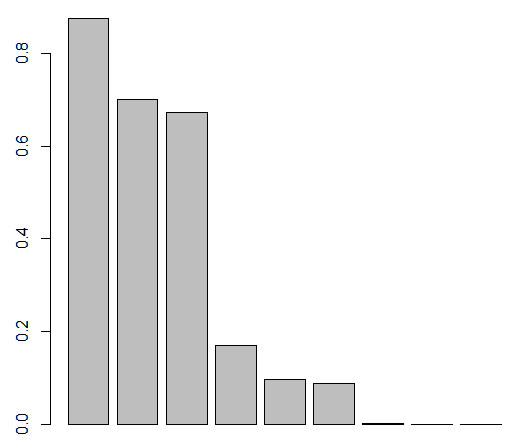
\includegraphics[width=.48\textwidth]{figures/Vandevoorde2-img63.png}\hfill%
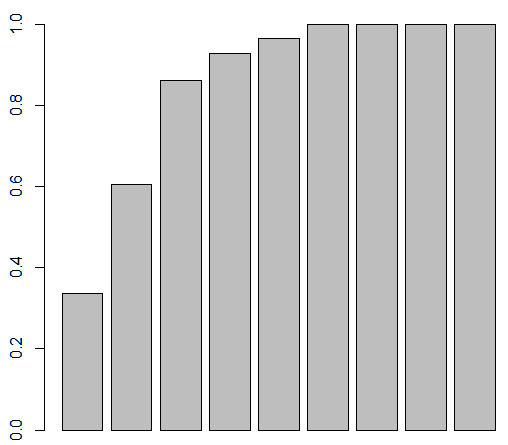
\includegraphics[width=.48\textwidth]{figures/Vandevoorde2-img64.png}
\caption{\label{fig:4:62}Left: Scree plot for TransDutch\textsubscript{ENG}. Right: \label{fig:4:63}Cumulative scree plot for TransDutch\textsubscript{ENG}}
\end{figure}

A HAC was carried out on the output of the CA. The cut-off point was set at a height of 2, offering a cluster solution with 6 clusters.\footnote{Note that \texttt{–pvrect()} would have yielded the same cluster solution.} Cluster n°1 contains \textit{oprichten} `to establish' and \textit{opzetten} `to set up'; cluster n°2 includes \textit{aanvang} `commencement' and \textit{start} `start'; cluster n°3 comprises \textit{eerst} `firstly', \textit{van start gaan} `to take off', \textit{beginnen} `to begin', \textit{krijgen} `to get', \textit{starten} `to start', \textit{gaan} `to go', \textit{worden} `to become'; cluster n°4 contains \textit{komen} `to come' and \textit{opstarten} `to start up', cluster n°5 consists of \textit{ontstaan} `to come into being' and \textit{openen} `to open' and cluster n°6 contains \textit{begin} `beginning'. I consider the result presented in \figref{fig:4:64} as a possible visualization of a semantic field representing \textit{beginnen}/inchoativity in TransDutch\textsubscript{ENG}.

\begin{figure}
% 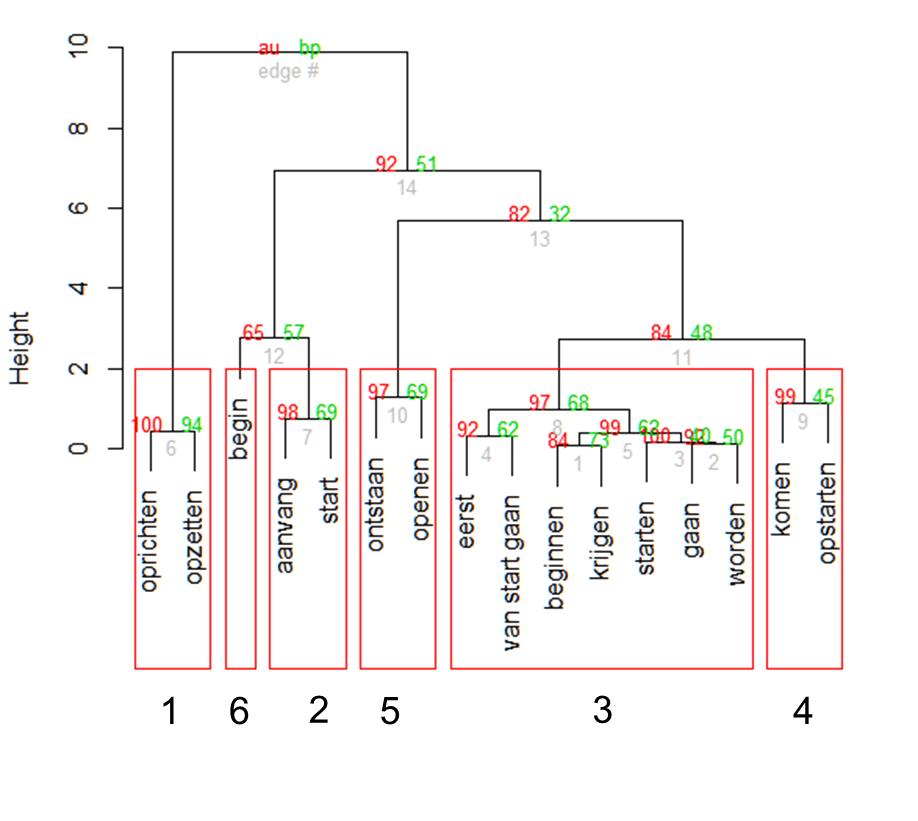
\includegraphics[height=.4\textheight]{figures/Vandevoorde2-img65.png}
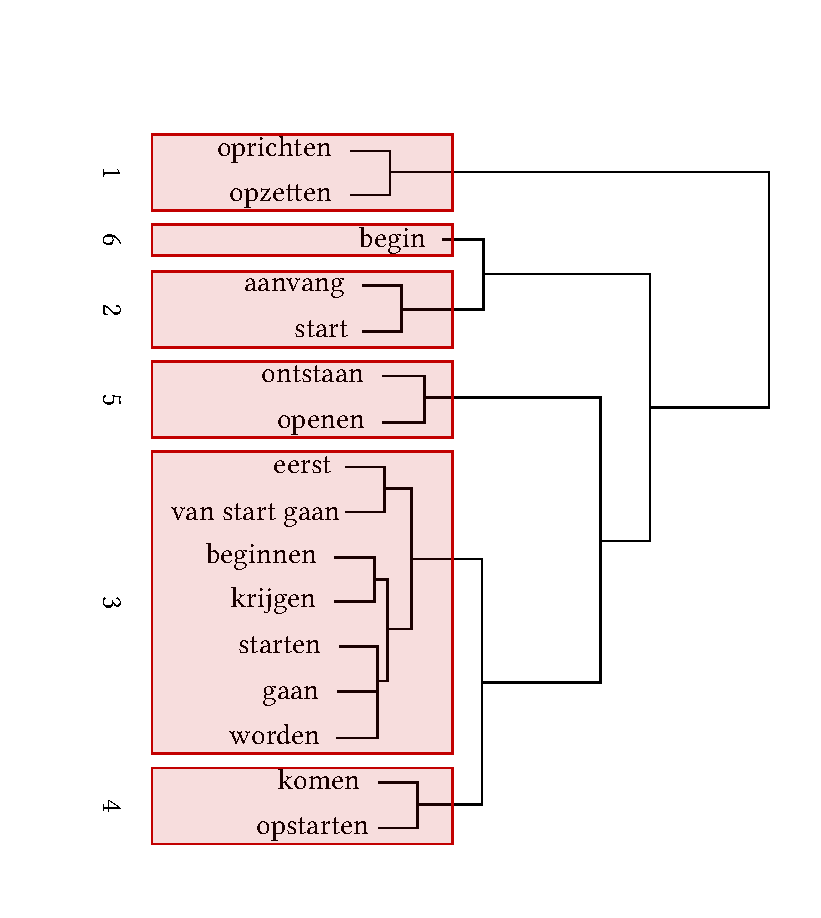
\includegraphics[width=.75\textwidth,trim=0 20 0 50]{figures/tree65.pdf}
\caption{\label{fig:4:64}Dendrogram representing a semantic field of \textit{beginnen}/inchoativity for TransDutch\textsubscript{ENG}}
\end{figure}

The chosen cluster solution was validated on the basis of the average silhouette width. For a solution with 6 clusters for TransDutch\textsubscript{ENG} I obtained an average silhouette width of 0.57, which I consider to indicate a good classification.

\begin{figure}
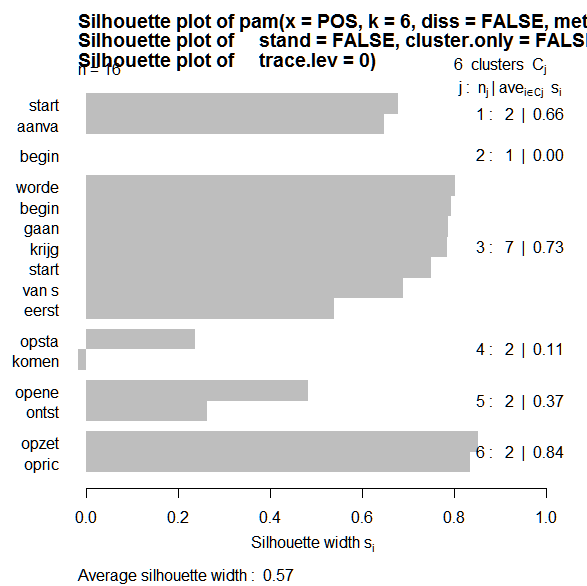
\includegraphics[height=.4\textheight]{figures/Vandevoorde2-img66.png}
\caption{\label{fig:4:65}Average silhouette width for cluster solution with 6 clusters for TransDutch\textsubscript{ENG}}
\end{figure}

A second validation was obtained via the calculation of a $k$-means clustering. When a cluster solution with 6 clusters is requested, $k$-means proposed the solution shown in \figref{fig:4:66} (the numeral beneath each lexeme assigns it to a specific cluster).

\begin{figure}
% 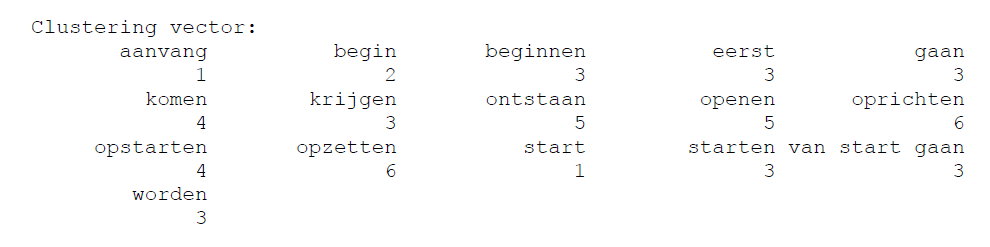
\includegraphics[width=\textwidth]{figures/Vandevoorde2-img67.png}
\begin{lstlisting}
Clustering vector:
      aanvang       begin    beginnen      eerst             gaan 
            1           2           3          3                3         
        komen     krijgen    ontstaan     openen        oprichten         
            4           3           5          5                6         
    opstarten    opzetten       start    starten   van start gaan         
            4           6           1          3                3         
       worden                                            
            3                                      
\end{lstlisting}
\caption{\label{fig:4:66}$k$-means clustering with 6 clusters for TransDutch\textsubscript{ENG}}
\end{figure}

The cluster solution proposed by the $k$-means clustering with 6 clusters is identical to the output of the HAC. On the basis of both validation techniques, it was concluded that the chosen cluster solution for TransDutch\textsubscript{ENG} is a good classification.

\subsection{Prototype-based organization of the clusters in the dendrogram (semasiological level)}
\label{sec:4.3.2}  
The centroid of each cluster was calculated and its distance to the zero-point of the semantic space was assessed by mapping the centroids onto a dot chart (\figref{fig:4:68} right). The content of each cluster number in the dot chart was summarized in the table accompanying \figref{fig:4:68} (right).\footnote{Parallel to SourceDutch, the numerals on the y-axis of the dot chart in \figref{fig:4:68} (right) are assigned by a previously established list (based on the output of the cluster analysis), necessary to calculate the cluster centroid (the order of the assigned numerals is arbitrary).}

\begin{figure} 
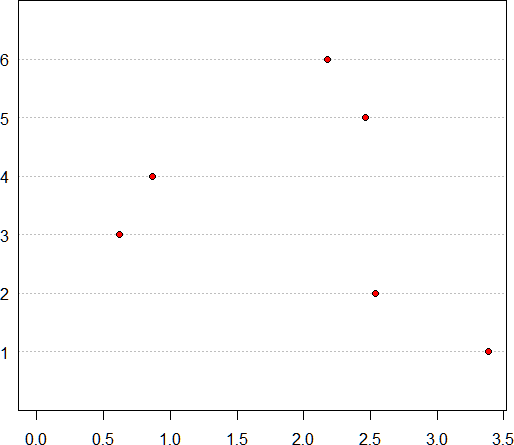
\includegraphics[height=.4\textheight]{figures/Vandevoorde2-img68.png}
\scriptsize
\begin{tabular}{l>{\itshape}l}
\lsptoprule
Cluster 1 & aanvang{\normalfont,} start\\
Cluster 2 & begin\\
Cluster 3 & beginnen{\normalfont,} eerst{\normalfont,} gaan{\normalfont,} krijgen{\normalfont,} starten{\normalfont,} van start gaan{\normalfont,} worden\\
Cluster 4 & komen{\normalfont,} opstarten\\
Cluster 5 & ontstaan{\normalfont,} openen\\
Cluster 6 & oprichten{\normalfont,} opzetten\\
\lspbottomrule
\end{tabular}
\normalsize
\caption{\label{fig:4:kmeansdutch6}Dot chart presenting the distance of the cluster centroids to the zero-point of the semantic space of TransDutch\textsubscript{ENG}}
\end{figure}

The dot chart shows that cluster n°3, containing \textit{beginnen}, \textit{eerst}, \textit{gaan}, \textit{krijgen}, \textit{starten}, \textit{van start gaan} and \textit{worden} is the central cluster in the analysis, closely followed by cluster n°4 with \textit{komen} and \textit{opstarten}. Clusters n°6 with \textit{begin}, n°5 with \textit{ontstaan} and \textit{openen} and n°2 with \textit{aanvang} and \textit{start} are situated closely together, but further away from the plot’s origin. Cluster n°1 comprising \textit{oprichten} and \textit{opzetten} is the most peripheral cluster.

\subsection{Prototype-based organization of the lexemes within each cluster (onomasiological level)}
\label{sec:4.3.3}  
The prototype-based organization of the lexemes within each cluster was examined by measuring the distance of the lexemes within each cluster to the centroid of the cluster they belong to, as well as by calculating the medoid of each cluster. Both measures were used to determine which lexical item can be considered as the most prototypical expression of the cluster it belongs to.

\subsubsection{Centroids}
\label{sec:4.3.3.1}  
The dot charts in Figures~\ref{fig:4:67}--\ref{fig:4:72} represent the distance of all the lexemes to the centroid (the abstraction of the prototype) of a particular cluster.

\begin{figure}
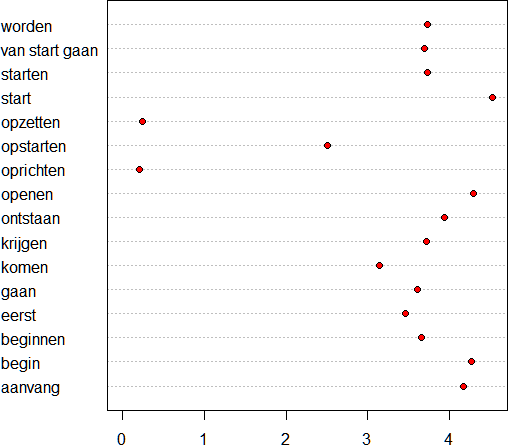
\includegraphics[width=.48\textwidth,trim=0 10 0 10]{figures/Vandevoorde2-img69.png}\hfill%
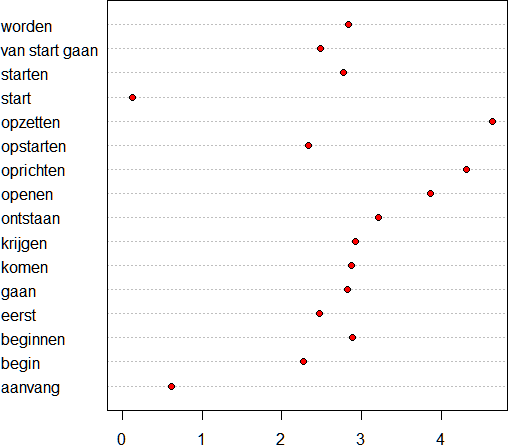
\includegraphics[width=.48\textwidth,trim=0 10 0 10]{figures/Vandevoorde2-img70.png}
\caption{\label{fig:4:67}Cluster n°1 (left) and n°2 (right) for TransDutch\textsubscript{ENG}\label{fig:4:68}}
\end{figure}

\begin{figure}
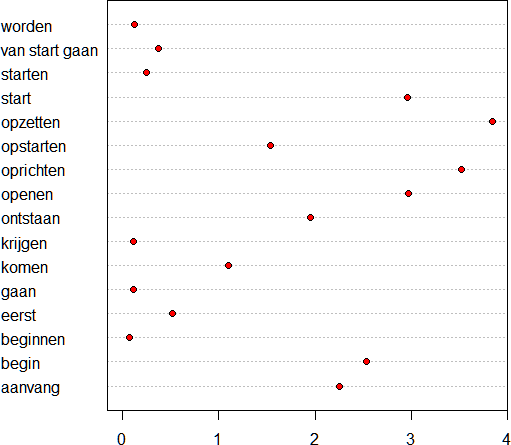
\includegraphics[width=.48\textwidth,trim=0 10 0 10]{figures/Vandevoorde2-img71.png}\hfill%
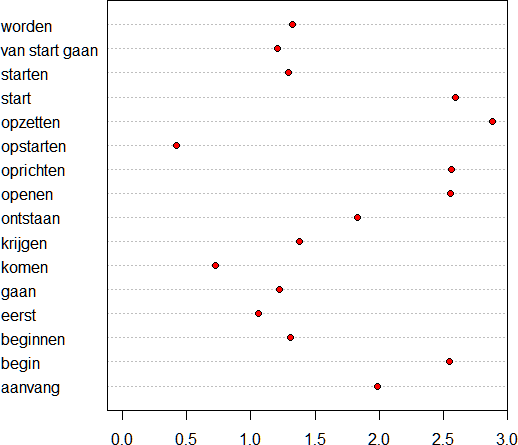
\includegraphics[width=.48\textwidth,trim=0 10 0 10]{figures/Vandevoorde2-img72.png}
\caption{\label{fig:4:69}Cluster n°3 (left) and n°4 (right) for TransDutch\textsubscript{ENG}\label{fig:4:70}}
\end{figure}

\begin{figure}                                              
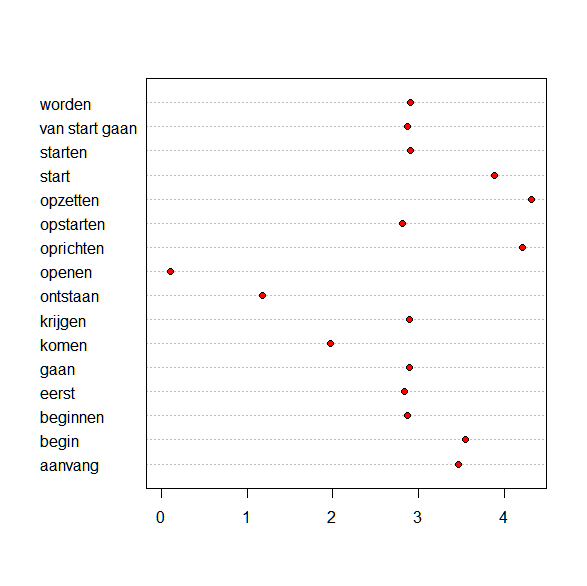
\includegraphics[width=.48\textwidth,trim=0 10 0 10]{figures/Vandevoorde2-img73.png}\hfill%
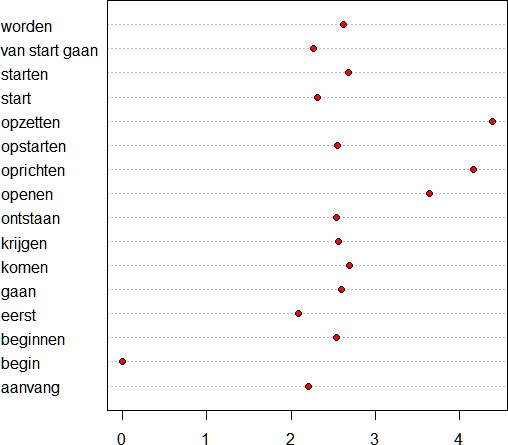
\includegraphics[width=.48\textwidth,trim=0 10 0 10]{figures/Vandevoorde2-img74.png}
\caption{\label{fig:4:71}Cluster n°5 (left) and n°6 (right) for TransDutch\textsubscript{ENG}\label{fig:4:72}}
\end{figure}

Just as for SourceDutch, the differences in distance of the lexemes to their cluster’s centroid is often very small, so I again used the calculated distances whenever the dot charts did not clearly indicate which lexeme is the closest one to the centroid (see \tabref{appendix-table-I}, Appendix~\ref{ch:C}).

The calculated distances for cluster n°1, show that \textit{oprichten} is slightly closer to the cluster’s centroid (0.2004520) than \textit{opzetten} (0.2476172). As for cluster n°2, \textit{start} is the lexeme closest to the centroid of the cluster. In cluster n°3, \textit{beginnen} (0.06521312) is closer to the centroid than \textit{gaan} (0.11345029), \textit{krijgen} (0.11370695) and \textit{worden} (0.12738579). For cluster n°4, \textit{opstarten} is undoubtedly the closest lexeme to the centroids of the cluster. The second lexeme in cluster n°4, \textit{komen} is situated as close to \textit{opstarten} (of cluster n°4) as it is to \textit{eerst} (of cluster n°3), and also quite close to a number of other lexemes pertaining to cluster n°3. This implies that the clustering of \textit{komen} with \textit{opstarten} is not so clear cut. Looking back at cluster n°3, \textit{komen} is indeed the lexeme that is situated closest to the lexemes of cluster n°3. For cluster n°5, it is \textit{openen} which situates itself closest to the cluster centroids. For cluster n°6, there is no need to determine the best representation of the abstraction of the prototype since it is a singleton cluster with \textit{begin}.

\subsubsection{Medoids}
\label{sec:4.3.3.2}  
\tabref{tab:4:15} below shows the calculated medoid for cluster n°3 and compares it with the lexemes closest to the centroid of the cluster (all other clusters contain either two lexemes or only one, so the medoid could not be calculated).

\begin{table}
\caption{\label{tab:4:15}Comparison of medoids and lexemes closest to the centroids for TransDutch\textsubscript{ENG}}
\begin{tabularx}{\textwidth}{XXl} 
\lsptoprule
& Medoid & Lexeme closest to centroids\\
\midrule
Cluster n°3 &\itshape worden &\itshape beginnen\\
\lspbottomrule
\end{tabularx}
\end{table}

The medoid and the closest lexeme to the centroid of cluster n°3 do not coincide. In addition, the difference in distance to the centroid between the first and the second lexeme points, to a lesser extent than in SourceDutch, towards the presumed ``competition'' between several more central expressions within the cluster: for cluster n°3, \textit{beginnen} is now closely followed by \textit{gaan}, \textit{krijgen} and worden. \textit{Starten} – for which a more central position in the cluster was expected – is situated slightly further away.

\subsection{Interpretation of the semantic field of beginnen\textit{/}inchoativity for TransDutch\textsubscript{ENG}}\label{sec:4.3.4}  
The following interpretation of a semantic field of \textit{beginnen}/inchoativity for\linebreak TransDutch\textsubscript{ENG} includes the assignment of a meta-label for each meaning distinction. The specific meaning distinctions determined for SourceDutch will be used as a point of reference to interpret the field of TransDutch\textsubscript{ENG}. I will consequently attempt to assign the meta-labels that were chosen on the basis of the SourceDutch field to the field of TransDutch\textsubscript{ENG}.

Cluster n°3 can be considered as the most central cluster or \textsc{reference cluster}, representing the idea of \textsc{general onset}. Parallel to SourceDutch, this is substantiated on both the semasiological and the onomasiological level. On the semasiological level, the centroid of cluster n°3 is the closest one to the origin of the semantic space (considered as the prototypical center). On the onomasiological level, the distances of the lexemes of cluster n°3 to each of the centroids of the other clusters (depicted in Figures~\ref{fig:4:67}--\ref{fig:4:72}) are always fairly equal (with the exception of cluster n°4). This implies that cluster n°3 shows the least deviation with respect to the other clusters (equally similar to the abstract prototype of each of the other clusters). In addition, the initial lexeme \textit{beginnen} (considered as the most prototypical expression of inchoativity) can be found within the \textsc{reference cluster}, strengthening my assumption that this cluster is holding the most prototypical expressions of inchoativity. The \textsc{reference cluster} has furthermore become larger compared to SourceDutch: \textit{eerst} – which held a peripheral position in SourceDutch (outliers are often depicted as singleton clusters in a HAC) – is now part of the \textsc{reference cluster}, as well as \textit{krijgen} and \textit{worden}, labeled as {\textsc{non-lexicalized inchoativity}} in SourceDutch. This implies that more peripheral expressions of inchoativity as well as expressions where inchoativity is non-lexicalized are used more prominently to express inchoativity in TransDutch\textsubscript{ENG}, compared to SourceDutch.

Just as for SourceDutch, I will now further inspect the different sub-nodes of the \textsc{reference cluster}, to see whether the same meaning distinction between \textsc{action} and \textsc{state after onset} is also present in TransDutch\textsubscript{ENG}. I observe three sub-nodes, one higher subnode with \textit{eerst} and \textit{van start gaan} and two lower sub-nodes of which one with \textit{beginnen} and \textit{krijgen} and a second one with \textit{starten}, \textit{gaan} and \textit{worden}. Whereas for SourceDutch, the subnodes of the \textsc{reference cluster} clearly laid bare a division between \textsc{action} and \textsc{state after onset}, this is no longer the case in TransDutch\textsubscript{ENG} (e.g. \textit{gaan} is clustered with \textit{starten}). At first sight, it seems that within the \textsc{reference cluster} of TransDutch\textsubscript{ENG}, the emphasis is on the wider relatedness between the verbs rather than on the division between \textsc{action} and \textsc{state after onset}. However, at the onomasiological level, \textit{beginnen} (0.06521312) is the closest lexeme to the centroid, followed by \textit{gaan} (0.11345029), which is considered as a \textsc{state after onset} verb, followed by two verbs labeled as {\textsc{non-lexicalized inchoativity}}, i.e. \textit{krijgen} (0.11370695) and \textit{worden} (0.12738579); followed by the \textsc{action} verbs \textit{starten} (0.25003812) and \textit{van start gaan} (0.37259612). Seen from this perspective, the ``confusion'' of \textsc{action} and \textsc{state after onset} verbs within the \textsc{reference cluster} is much less present than the dendrogram would seem to suggest. In TransDutch\textsubscript{ENG}, the competition between \textsc{action} and \textsc{state after onset} verbs has been breached by a more prominent use of verbs which do not lexicalize inchoativity.

Cluster n°4 is a somewhat odd, new cluster. The dot chart in \sectref{sec:4.3.2} revealed that this cluster is the closest one to the \textsc{reference cluster}, confirming its close relatedness to the latter. Since the \textsc{reference cluster} contains the \textsc{action} verbs as well as verbs of {\textsc{non-lexicalized inchoativity}}, one would have expected \textit{opstarten} and \textit{komen} in the \textsc{reference cluster} too. There are indeed a number of indications that cluster n°4 is very closely related to the \textsc{reference cluster}: (i) the lexemes of cluster n°4 seem to behave in a similar way to those of cluster n°3: the lexemes of both clusters keep a similar distance from the centroids of the other clusters, implying that they show very little deviation with respect to the other clusters (and the same amount of deviation for both clusters n°3 and n°4); (ii) with respect to the distance of the lexemes \textit{komen} and \textit{opstarten} to the lexemes of the \textsc{reference cluster} (\figref{fig:4:70} right), it can be observed that \textit{komen} (0.7203757) is as close to \textit{eerst} (1.0569324) as it is to \textit{opstarten} (0.4202192). Hence, it is mainly \textit{opstarten} that determines the separate clustering here (\textit{komen} holds a middle position between clusters n°3 and n°4). Recall that in SourceDutch, \textit{opstarten} already formed a significant sub-node within the \textsc{reference cluster}. This distinction now seems to be emphasized in TransDutch\textsubscript{ENG} by the separate clustering of \textit{opstarten}.

Cluster n°2 contains \textit{aanvang} and \textit{start}. Based on statistical significance, cluster n°6 – a singleton cluster with \textit{begin} – is connected in a higher (less significant) node to \textit{aanvang} and \textit{start}. The word-class dependent clustering observed for SourceDutch is maintained. On the semasiological level, the distance of the centroid of cluster n°2 and cluster n°6 to the zero-point of the semantic space shows that cluster n°6 (\textit{begin}) is much closer to the zero-point than cluster n°2, implying that in TransDutch\textsubscript{ENG}, \textit{begin} is a more central expression of inchoativity than \textit{aanvang} and \textit{start} are. In TransDutch\textsubscript{ENG}, the distance between \textit{aanvang} and \textit{start} is also larger (\figref{fig:4:68} right) compared to SourceDutch (\figref{fig:4:56} left).

The clustering within clusters n°1 (\textit{oprichten} with \textit{opzetten}) and n°5 (\textit{ontstaan} with \textit{openen}) have remained unaltered with respect to their corresponding clusters in SourceDutch. On the onomasiological level, the difference in distance to the centroid of the lexemes of cluster n°1 (\textit{oprichten} and \textit{opzetten}) has become larger in TransDutch\textsubscript{ENG}, compared to the corresponding cluster in SourceDutch. For cluster no°5, (\textit{ontstaan} and \textit{openen}) the difference in distance to the centroid has become smaller in TransDutch\textsubscript{ENG} compared to SourceDutch. \figref{fig:4:73} below now shows the semantic field of \textit{beginnen}/inchoativity for TransDutch\textsubscript{ENG} with the meta-labels.

\begin{figure}
% 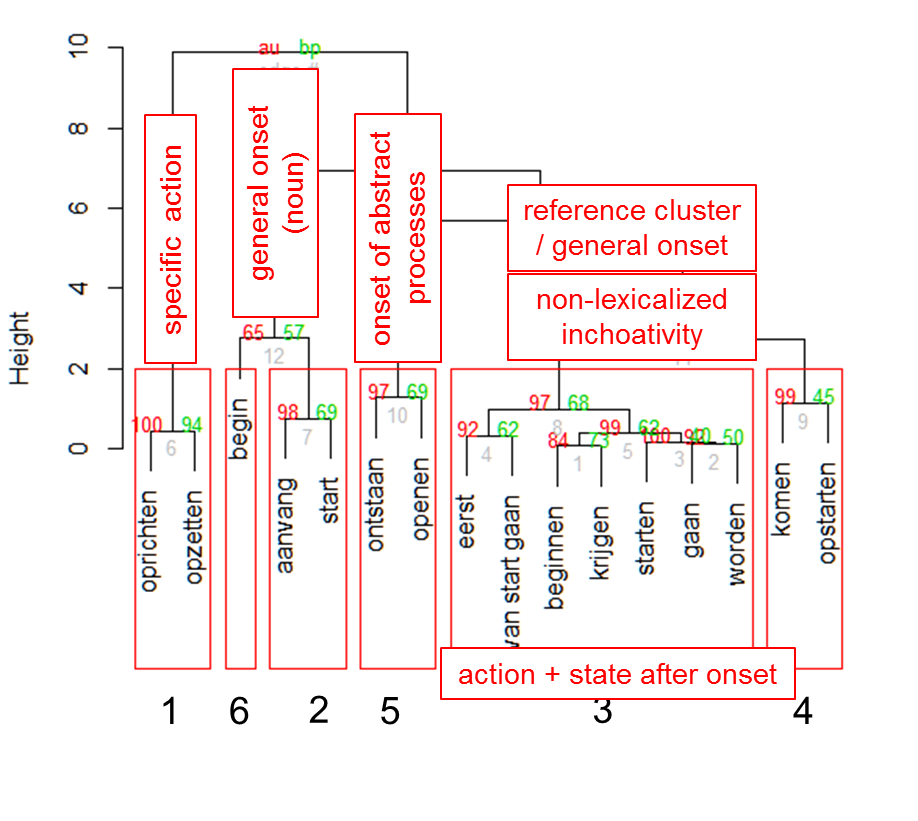
\includegraphics[height=.4\textheight]{figures/Vandevoorde2-img75.png}
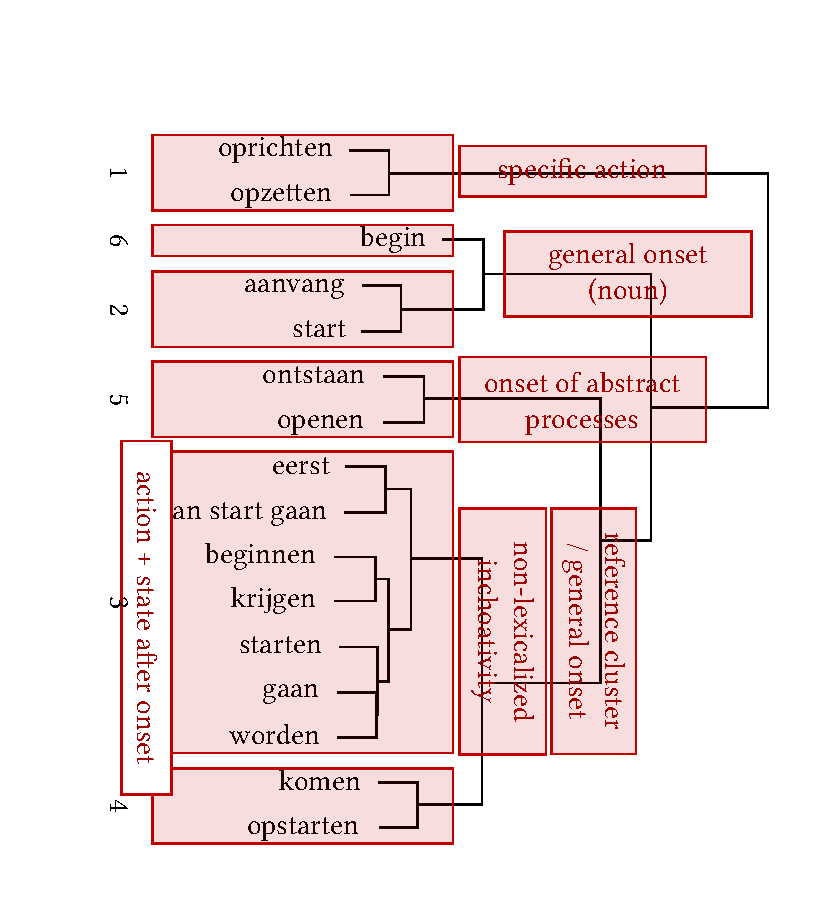
\includegraphics[width=.75\textwidth,trim=0 20 0 50]{figures/tree75.pdf}
\caption{\label{fig:4:73}Dendrogram representing a semantic field of \textit{beginnen}/inchoativity for TransDutch\textsubscript{ENG} with meta-labels}
\end{figure}

\section{TransDutch\textsubscript{FR}}
\label{sec:4.4}  
The interpretation of the visualization of TransDutch\textsubscript{FR} follows the same steps as for SourceDutch and TransDutch\textsubscript{ENG}.

\subsection{Results of the Hierarchical Agglomerative Cluster analysis}
\label{sec:4.4.1}  
Figure~\ref{fig:4:74} shows the distribution of the variation over the latent dimensions of the CA. On the basis of these scree plots, it was decided to reduce the number of dimensions of the CA to 4.

\begin{figure}
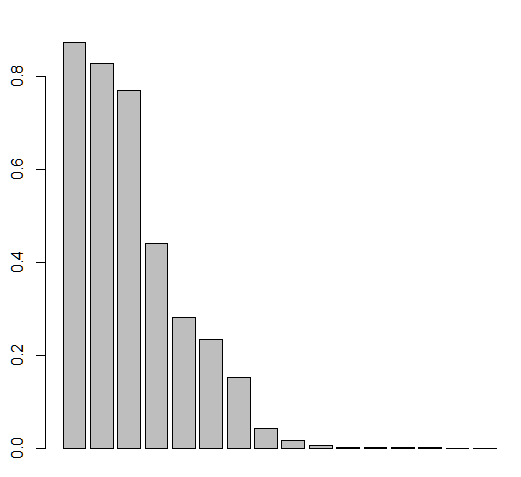
\includegraphics[width=.48\textwidth]{figures/Vandevoorde2-img76.png}\hfill%
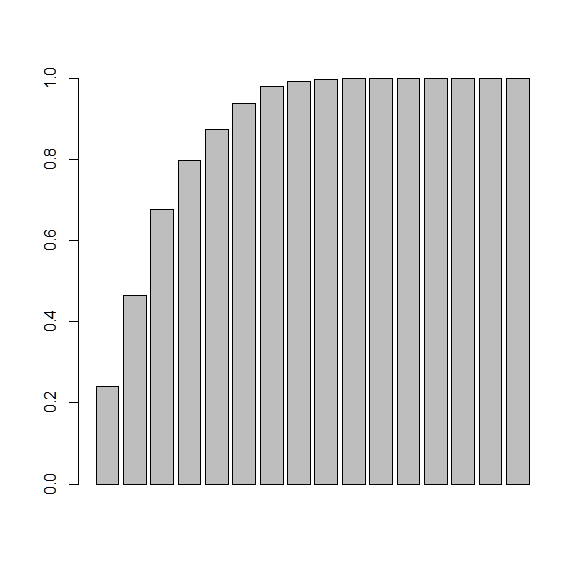
\includegraphics[width=.48\textwidth]{figures/Vandevoorde2-img77.png}
\caption{\label{fig:4:74}Left: Scree plot for TransDutch\textsubscript{FR}. \label{fig:4:75}Right: Cumulative scree plot for TransDutch\textsubscript{FR}}
\end{figure}

A HAC was carried out and a cut-off point at a height of 5 was chosen, rendering a cluster solution with 4 clusters. Cluster n°1 contains \textit{start} `start', \textit{aanvang} `commencement' and \textit{begin} `beginning'; cluster n°2 contains \textit{ontstaan} `to come into being' and \textit{openen} `to open'; cluster n°3 comprises \textit{opzetten} `to set up', \textit{oprichten} `to establish', \textit{opstarten} `to start up', \textit{starten} `to start' and \textit{van start gaan} `to take off'; cluster n°4 holds \textit{eerst} `firstly', \textit{gaan} `to go', \textit{beginnen} `to begin', \textit{worden} `to become', \textit{komen} `to come' and \textit{krijgen} `to get'.

The result presented in \figref{fig:4:76} is considered as a possible visualization of a semantic field representing \textit{beginnen}/inchoativity in TransDutch\textsubscript{FR}.

\begin{figure}
% 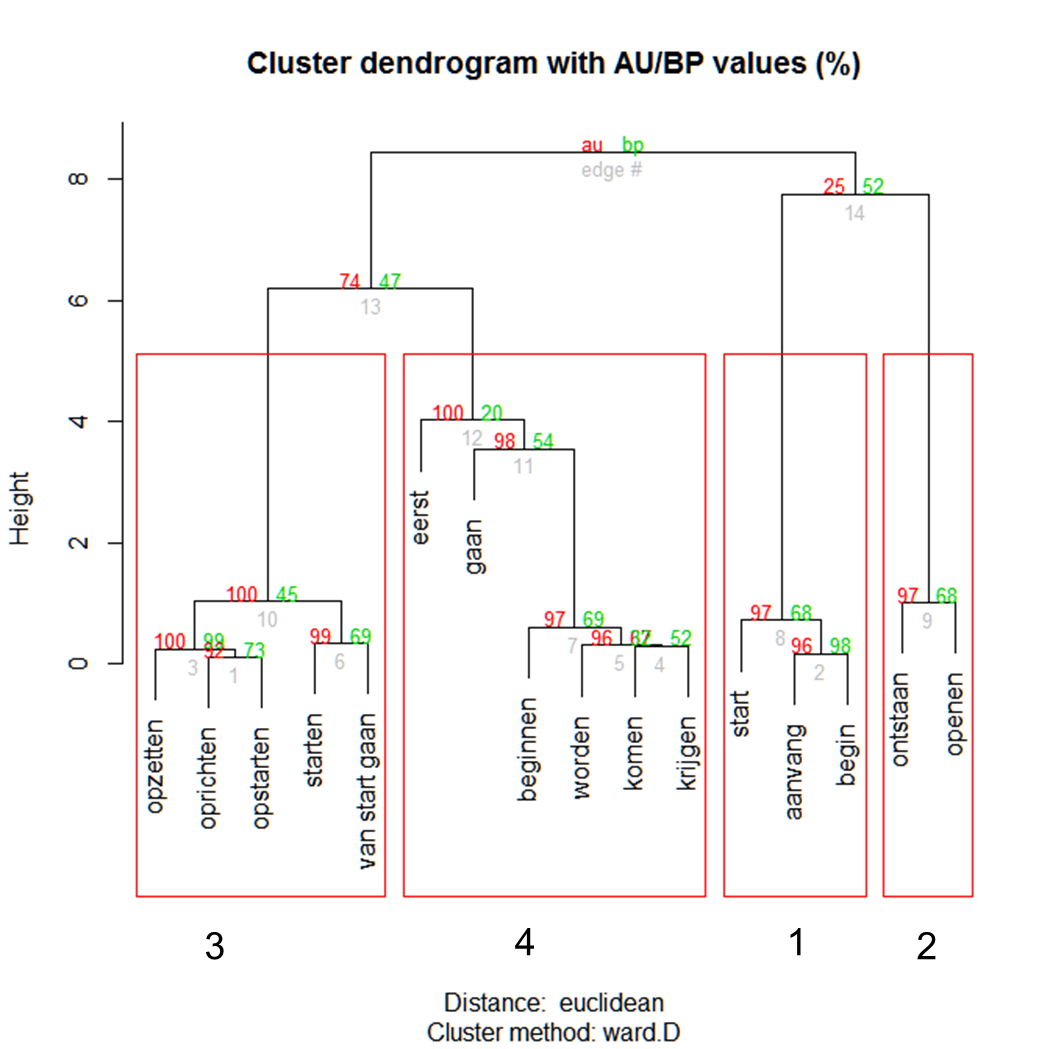
\includegraphics[height=.4\textheight]{figures/Vandevoorde2-img78.png}
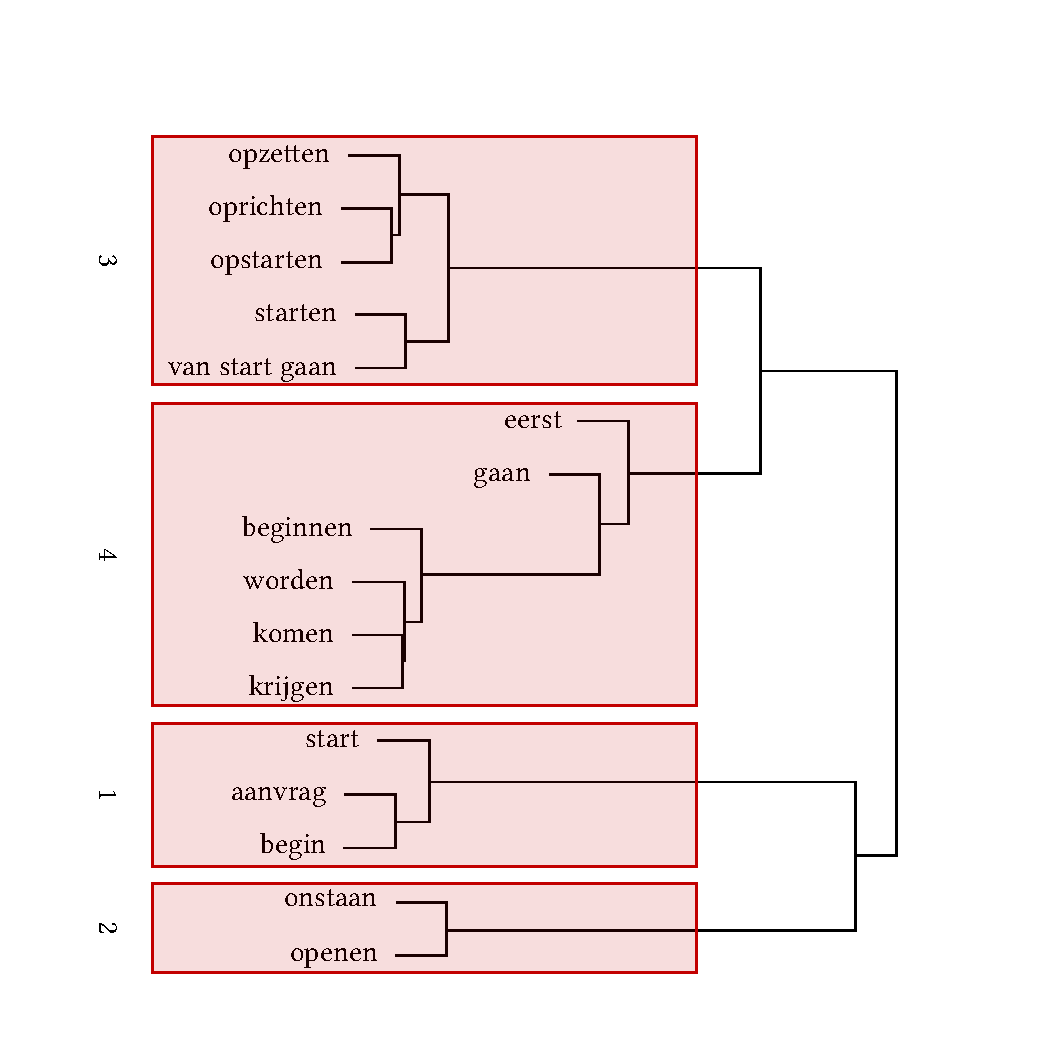
\includegraphics[width=.75\textwidth,trim=0 20 0 20]{figures/tree78.pdf}
\caption{\label{fig:4:76}Dendrogram representing a semantic field of \textit{beginnen}/inchoativity for TransDutch\textsubscript{FR}}
\end{figure}

The cluster solution is validated by the average silhouette width for a solution with 4 clusters (average silhouette width = 0.53) (\figref{fig:4:77}) and by the calculation of a $k$-means clustering with 4 clusters, which proposes an identical cluster solution to the output of the HAC as can be seen below (the numeral beneath each lexeme assigns it to a specific cluster). On the basis of both validation techniques, I conclude that the chosen cluster solution for TransDutch\textsubscript{FR} can be considered a good classification.

\begin{figure}
% 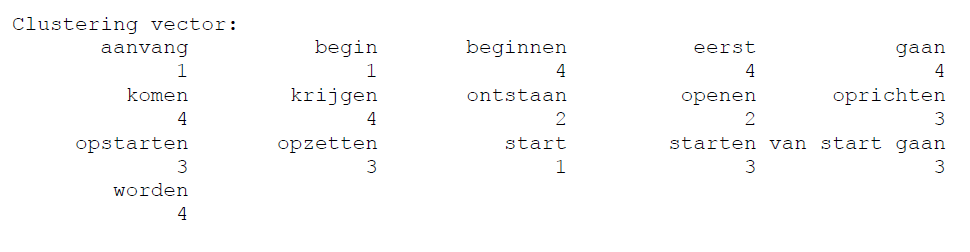
\includegraphics[width=\textwidth]{figures/Vandevoorde2-img79.png}
\begin{lstlisting}
Clustering vector:
      aanvang      begin    beginnen      eerst              gaan 
            1          1           4          4                 4
        komen    krijgen    ontstaan     openen         oprichten
            4          4           2          2                 3
    opstarten   opzetten       start    starten    van start gaan
            3          3           1          3                 3
       worden               
            3               
\end{lstlisting}
\caption{\label{fig:4:kmeansdutch4}$k$-means clustering with 4 clusters for TransDutch\textsubscript{FR}}
\end{figure}

\begin{figure}
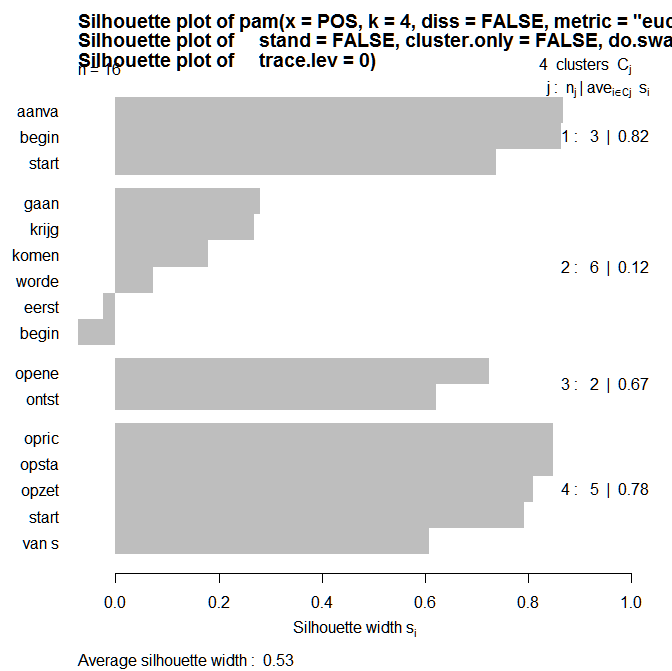
\includegraphics[height=.4\textheight]{figures/Vandevoorde2-img80.png}
\caption{\label{fig:4:77}Average silhouette width for cluster solution with 4 clusters for TransDutch\textsubscript{FR}}
\end{figure}

\subsection{Prototype-based organization of the clusters in the dendrogram (semasiological level)}
\label{sec:4.4.2}  
The distance from each cluster’s centroid to the zero-point of the semantic space is calculated and mapped on a dot chart (\figref{fig:4:78}). The content of each cluster number in the dot chart is summarized in the table accompanying \figref{fig:4:78}.

\begin{figure}
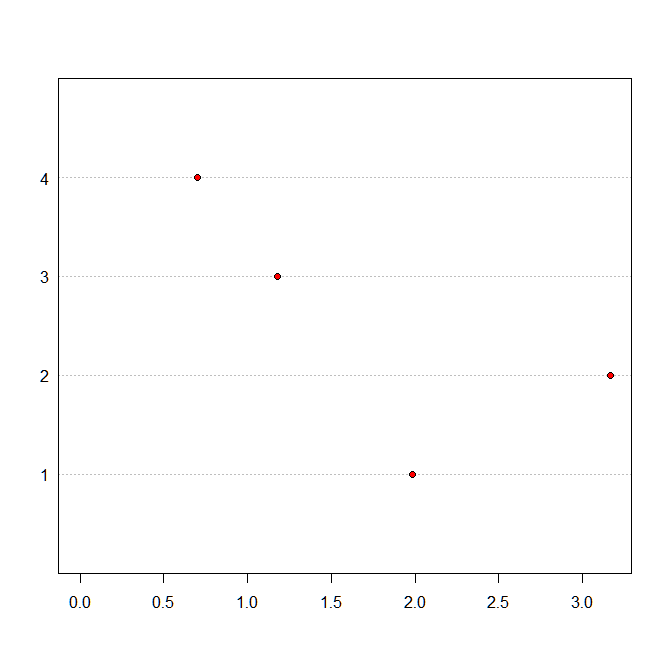
\includegraphics[height=.4\textheight]{figures/Vandevoorde2-img81.png}\vspace*{\baselineskip}
\scriptsize
\begin{tabular}{l>{\itshape}l}
\lsptoprule
Cluster 4 & eerst{\normalfont,} gaan{\normalfont,} beginnen{\normalfont,} komen{\normalfont,} worden{\normalfont,} krijgen\\
Cluster 3 & opzetten{\normalfont,} oprichten{\normalfont,} opstarten{\normalfont,} starten{\normalfont,} van start gaan\\
Cluster 2 & ontstaan{\normalfont,} openen\\
Cluster 1 & start{\normalfont,} aanvang{\normalfont,} begin\\
\lspbottomrule
\end{tabular}
\normalsize
\caption{\label{fig:4:78}Dot chart presenting the distance of the cluster centroids to the zero-point of the semantic space of TransDutch\textsubscript{FR}}
\end{figure}

Cluster n°4, containing \textit{eerst}, \textit{gaan}, \textit{beginnen}, \textit{komen}, \textit{worden}, \textit{krijgen} is the central cluster in the analysis since it is situated closest to the zero-point of the semantic space. Cluster n°3 with \textit{opzetten}, \textit{oprichten}, \textit{opstarten}, \textit{starten} and \textit{van start gaan} comes in second place and is followed by cluster n°1 (\textit{start}, \textit{aanvang}, \textit{begin}). The cluster that is furthest away from the zero-point of the semantic space is cluster n°2 comprising \textit{ontstaan} and \textit{openen}.

\subsection{Prototype-based organization of the lexemes within each cluster (onomasiological level)}
\label{sec:4.4.3}  
The prototype-based organization of the lexemes within each cluster is examined on the basis of the following measures: the distance of the lexemes within each cluster to the centroid of the cluster they belong to and the medoid of each cluster.


\subsubsection{Centroids}
\label{sec:4.4.3.1}  
The dot charts in Figures~\ref{fig:4:79}--\ref{fig:4:82} represent the distances of all the lexemes in the analysis to the centroid of one particular cluster. I again used the calculated distances (which are represented by the dots in the dot charts) to evaluate the distances to the centroids (see \tabref{appendix-table-J}, Appendix~\ref{ch:C}).

For cluster n°1, \textit{begin} is the closest lexeme to the centroid, situated at 0.05884857 of the centroid, followed by \textit{aanvang} at 0.12955053 and \textit{start} at 0.54160901 of the centroid. For cluster n°2, it is clear that \textit{openen} is the lexeme closest to the centroid of its cluster. As for cluster n°3, it is difficult to determine with the bare eye whether \textit{starten} (0.1160007) or \textit{oprichten} (0.2037736) is the lexeme closest to the centroid, but based on the calculated distances, I conclude that \textit{starten} is the closest one to the centroid of the cluster. Finally, for cluster n°4, \textit{beginnen} is the lexeme closest to the cluster’s centroid (0.6576414), followed by \textit{krijgen} (0.9121243). It is worthy to note here that the closest lexeme to the \textsc{reference cluster}, \textit{beginnen}, is situated at a relatively large distance from its cluster’s centroid (0.6576414). The distance of \textit{beginnen} to the centroid of the \textsc{reference cluster} it belongs to is the smallest for TransDutch\textsubscript{ENG} (0.06521312) and the largest for TransDutch\textsubscript{FR} (0.6576414); for SourceDutch it is 0.1254173.

\begin{figure}
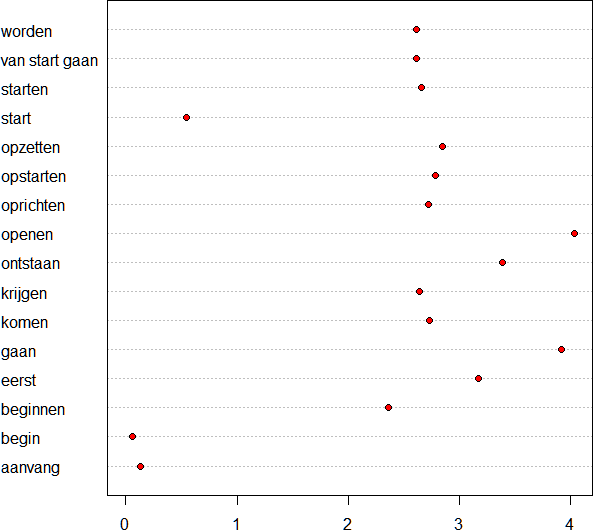
\includegraphics[width=.48\textwidth,trim=0 0 0 10]{figures/Vandevoorde2-img82.png}\hfill%
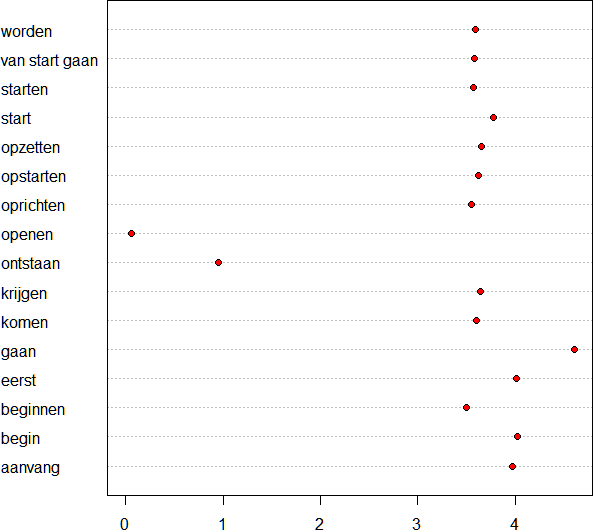
\includegraphics[width=.48\textwidth,trim=0 0 0 10]{figures/Vandevoorde2-img83.png}
\caption{\label{fig:4:79}Cluster n°1 (left) and n°2 (right) for TransDutch\textsubscript{FR}\label{fig:4:80}}
\end{figure}

\begin{figure}
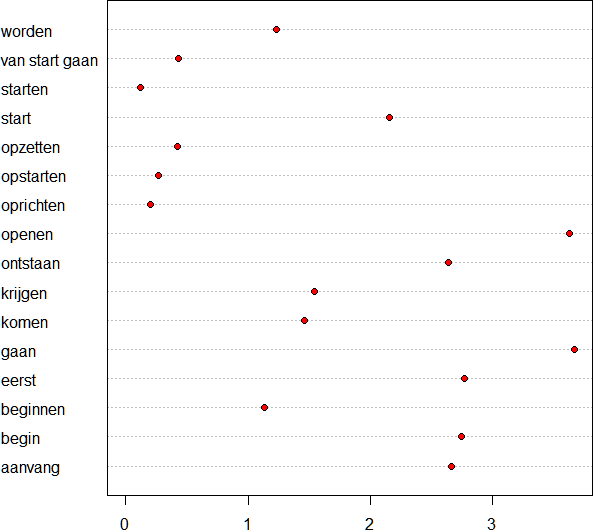
\includegraphics[width=.48\textwidth,trim=0 10 0 10]{figures/Vandevoorde2-img84.png}\hfill%
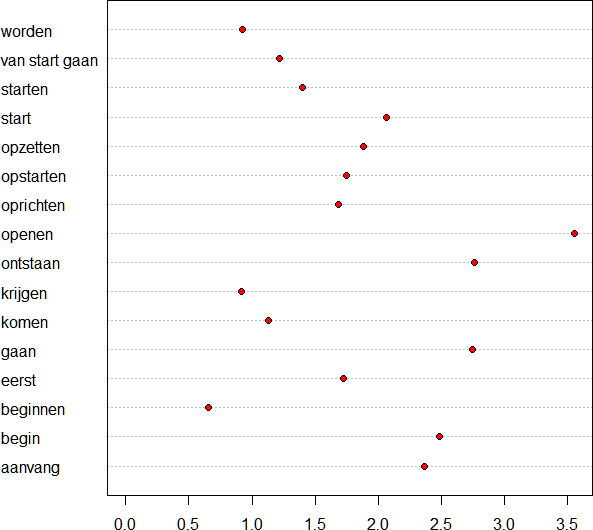
\includegraphics[width=.48\textwidth,trim=0 10 0 10]{figures/Vandevoorde2-img85.png}
\caption{\label{fig:4:81}Cluster n°3 (left) and n°4 (right) for TransDutch\textsubscript{FR}\label{fig:4:82}}
\end{figure}

\subsubsection{Medoids}
\label{sec:4.4.3.2}  
In \tabref{tab:4:16}, the lexemes closest to the centroid of clusters n°1, 3 and 4 are compared to their respective medoid.

\begin{table}
\caption{\label{tab:4:16}Comparison of medoids and lexemes closest to the centroids for TransDutch\textsubscript{FR}.}
\begin{tabularx}{\textwidth}{XXl}
\lsptoprule
& Medoid & Lexeme closest to centroids\\
\midrule 
Cluster n°1 & \itshape aanvang   & \itshape begin\\
Cluster n°3 & \itshape oprichten & \itshape starten\\
Cluster n°4 & \itshape krijgen   & \itshape beginnen\\
\lspbottomrule
\end{tabularx}
\end{table}

For TransDutch\textsubscript{FR}, the medoid and the lexeme closest to the centroid never coincide. What is striking is that the medoid is each time the second closest lexeme to the centroid of the cluster, an observation that was also made for a number of clusters of SourceDutch. Moreover, the medoids of clusters n°3 and n°4 indicate one meaning distinction: \textit{oprichten} in cluster n°3 refers to {\textsc{specific}} \textsc{action} and \textit{krijgen} in cluster n°4 refers to {\textsc{non-lexicalized inchoativity}}. For the same clusters, the lexemes closest to the centroids indicate a different meaning distinction within the same cluster: \textsc{action} for cluster n°3 (\textit{starten}) and \textsc{state after onset} for cluster n°4 (\textit{beginnen}).

\subsection{Interpretation of the semantic field of \textit{beginnen/}inchoativity for TransDutch\textsubscript{FR}}
\label{sec:4.4.4}  
In the following interpretation of a semantic field of \textit{beginnen}/inchoativity for TransDutch\textsubscript{FR}, the specific meaning distinctions determined for SourceDutch will again be used as a point of reference. Just as for TransDutch\textsubscript{ENG}, I will attempt to assign these meta-labels to the field of TransDutch\textsubscript{FR}.

Cluster n°4 is considered as the most central cluster in the dendrogram, representing the idea of \textsc{general onset}. As I showed in \sectref{sec:4.4.2}, its centroid is the closest one to the zero-point of the semantic space, considered as the prototypical center of the semantic space (semasiological level). Just as for SourceDutch and TransDutch\textsubscript{ENG}, \textit{beginnen} is part of the \textsc{reference cluster}, leading to the assumption that this cluster contains the most prototypical expressions of inchoativity. Parallel to TransDutch\textsubscript{ENG}, the number of lexemes in the \textsc{reference cluster} has increased compared to SourceDutch (5 lexemes in the \textsc{reference cluster} of SourceDutch, 7 for TransDutch\textsubscript{ENG} and 6 for TransDutch\textsubscript{FR}) (onomasiological level). Just as for TransDutch\textsubscript{ENG}, \textit{eerst} – which held a more peripheral position in SourceDutch – and the verbs \textit{komen}, \textit{krijgen} and \textit{worden} ({\textsc{non-lexicalized inchoativity}}) are now also part of the \textsc{reference cluster}. For both the TransDutch fields, more peripheral expressions of inchoativity as well as verbs which do not lexicalize inchoativity are used more prominently to express inchoativity compared to SourceDutch. Within the \textsc{reference cluster}, two significant terminal nodes (\textit{eerst} and \textit{gaan}) can be discerned, and one significant sub-node with four leaves with \textit{beginnen} as a significant terminal node within the sub-node and a second, underlying sub-node (also significant) with the three verbs labeled as {\textsc{non-lexicalized inchoativity}}. Within this \textsc{reference cluster}, the meaning distinctions \textsc{state after onset} and {\textsc{non-lexicalized inchoativity}} are both present. An important difference with SourceDutch and TransDutch\textsubscript{ENG} is that the \textsc{reference cluster} of TransDutch\textsubscript{FR} no longer contains any of the \textsc{action} verbs but only \textsc{state after onset} verbs (\textit{beginnen} and \textit{gaan}). Recall that in SourceDutch, \textsc{action} and \textsc{state after onset} verbs formed different meaning distinctions in the \textsc{reference cluster}, and that for TransDutch\textsubscript{ENG}, this distinction was still present in the \textsc{reference cluster} although less clear (see \sectref{sec:4.2.4}).

Cluster n°3 contains two significant sub-nodes, one with \textit{starten} and \textit{van start gaan}, the other one with \textit{oprichten}, \textit{opzetten}, \textit{opstarten}. Within cluster n°3 two meaning distinctions can be discerned: {\textsc{specific}} \textsc{action} (\textit{oprichten} and \textit{opzetten}) as well as \textsc{action} (\textit{starten} and \textit{van start gaan}). In TransDutch\textsubscript{FR}, the distinction between \textsc{action} and \textsc{state after onset} verbs is marked more clearly, compared to both SourceDutch and TransDutch\textsubscript{ENG}: the clustering of the \textsc{action} verbs with the verbs of {\textsc{specific}} \textsc{action} seems to emphasize the dynamic nature of these verbs. In addition, \textit{opstarten} (which formed a separate sub-node in the \textsc{reference cluster} of SourceDutch and a separate cluster in TransDutch\textsubscript{ENG}) is now part of the sub-node with \textit{oprichten} and \textit{opzetten}, emphasizing the relatedness of \textit{opstarten} to the specific contexts in which \textit{opzetten} and \textit{oprichten} are used, i.e. business-like activities. These contexts are confirmed for \textit{opstarten} by both examples in Cornetto \textit{een nieuw bedrijf in de V.S. opstarten} `to start up a new company in the U.S.' and by corpus examples (\ref{ex:15} and \ref{ex:16}) from the DPC:

\ea(dpc-arc-002049-nl, my emphasis)\label{ex:15}\\
Toen de buizenfabriek van Kimanis in augustus \Highlight{opgestart} werd, [...].\smallskip\\\relax
\textsc{target:} `When the pipe manufacturing facility in Kimanis was \Highlight{started up} in August, [...].'
\ex(dpc-vla-001161-nl, my emphasis)\label{ex:16}\\
In sterk ontwikkelde economieën worden bedrijven vooral \Highlight{opgestart} wegens een (markt)opportuniteit.\smallskip\\\relax
\textsc{target:} `Companies in highly developed economies are usually \Highlight{started up} on the basis of a (market) opportunity.' 
\z

On the semasiological level, the centroid for cluster n°3 is the second closest one to the zero-point of the semantic space. Its centroid is also situated fairly close to the centroid of cluster n°4, the \textsc{reference cluster}, which seems to confirm the close relationship between the two clusters and the proximity of cluster n°3 to the \textsc{reference cluster}. The proximity between cluster n°3 and cluster n°4 is further confirmed on the onomasiological level. The distance of the lexemes to the centroid of either cluster (Figure~\ref{fig:4:81}), shows a quite different image from the other clusters. In general, the lexemes pertaining to the cluster of which the centroid is taken as the zero-point are clearly closer to the centroid of their own cluster compared to the other lexemes not pertaining to the cluster. For the lexemes pertaining to clusters n°3 and n°4, the dot charts do not (as) clearly differentiate the lexemes pertaining to their own cluster from those pertaining to the other cluster: a number of lexemes are indeed at a fairly equal distance from both the centroids of cluster n°3 and cluster n°4 (see e.g. \textit{komen} is situated at 1.4586546 from the centroid of cluster n°3 and at 1.1315485 from the centroid of cluster n°4). The close relatedness between clusters n°3 and n°4 is not a total surprise since these clusters contain the \textsc{action} verbs in cluster n°3 and the \textsc{state after onset} verbs in cluster n°4 (which in SourceDutch and TransDutch\textsubscript{ENG} were separate sub-nodes of their \textsc{reference clusters}). Conclusively, the lexemes that were covered under the meta-label \textsc{reference cluster}\textit{/}\textsc{general onset} are now spread over two clusters according to the additional meaning distinction \textsc{action}\slash \textsc{state after onset}. Both cluster n°3 and cluster n°4 also contain an additional meta-label, i.e. {\textsc{specific}} \textsc{action} for cluster n°3 and {\textsc{non-lexicalized inchoativity}} for cluster n°4.

Cluster n°1 contains the nouns \textit{start}, \textit{aanvang} and \textit{begin}. Just as in SourceDutch, all three nouns are now again part of one, significant cluster. The centroid of cluster n°1 is closely following the centroid of clusters n°3 and n°4 (\figref{fig:4:78}), confirming the relatedness of this cluster of nouns to the two more central clusters (semasiological level). Note that the only three nouns in the set of lexemes are again clustered together, confirming again the word-class dependent clustering. In addition, the distance from the lexemes to their cluster’s centroid shows that \textit{begin} and \textit{aanvang} are the closest to the centroid, \textit{start} is situated considerably further away. Although the overall clustering of the three lexemes into one meaning distinction is similar to SourceDutch, the distance from the lexemes to their cluster’s centroids is different as small differences on the onomasiological level are observed: for SourceDutch, \textit{start} and \textit{begin} are competing to be the closest lexeme to the centroid, with \textit{aanvang} situated somewhat further away, whereas in TransDutch\textsubscript{FR}, \textit{aanvang} is much closer to \textit{begin} (the closest lexeme to the centroid) and \textit{start} is situated further away. The situation is also very different from that for TransDutch\textsubscript{ENG}, where \textit{begin} formed a new, singleton cluster, and \textit{aanvang} and \textit{start} were clustered together.

Finally, cluster n°2 contains \textit{ontstaan} and \textit{openen}. This is the only cluster that has remained unaltered throughout SourceDutch, TransDutch\textsubscript{FR} and Trans-\linebreak Dutch\textsubscript{ENG}. The distance from the two lexemes to the centroids of their cluster remains also fairly equal throughout the three visualizations. \figref{fig:4:83} shows the semantic field of \textit{beginnen} for TransDutch\textsubscript{FR} with integration of the meta-labels.

\begin{figure}
% 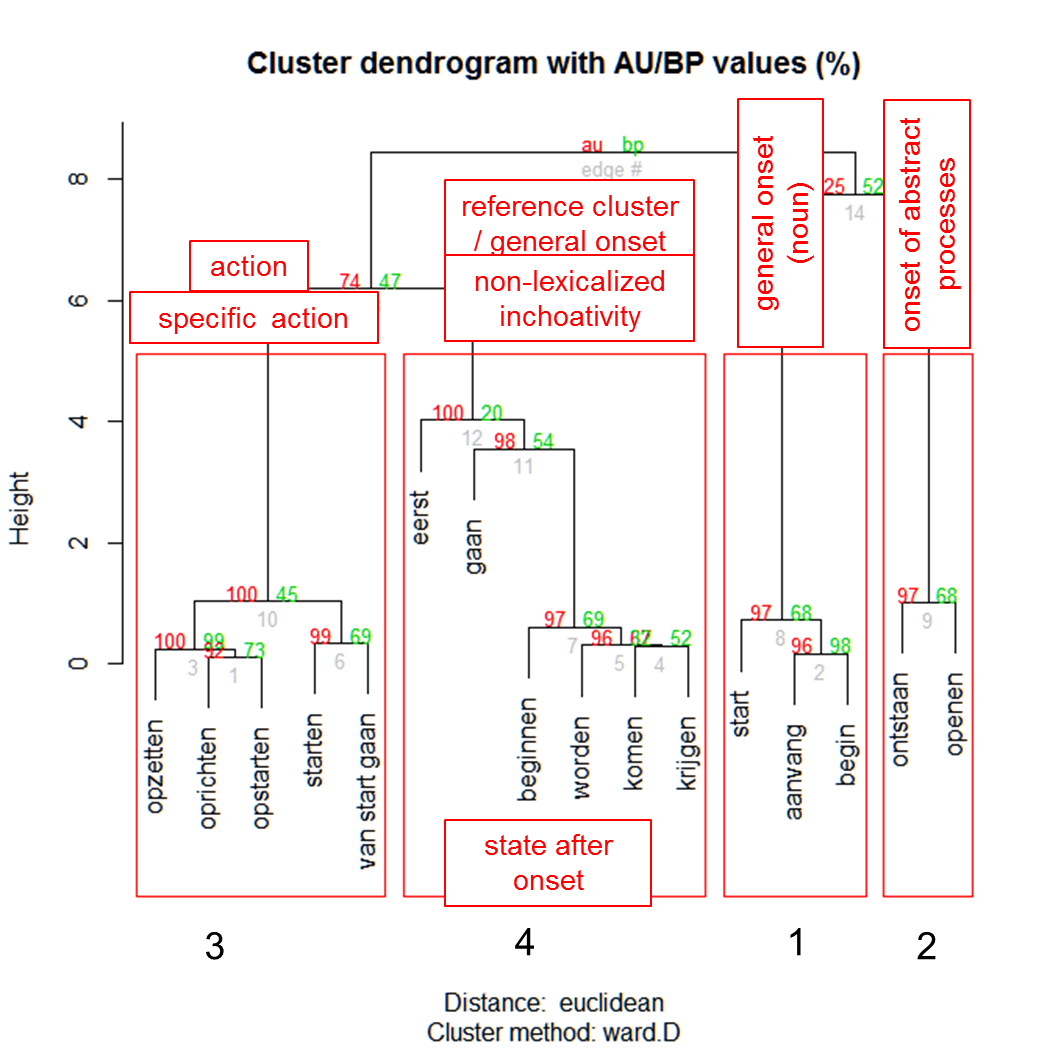
\includegraphics[height=.4\textheight]{figures/Vandevoorde2-img86.png}
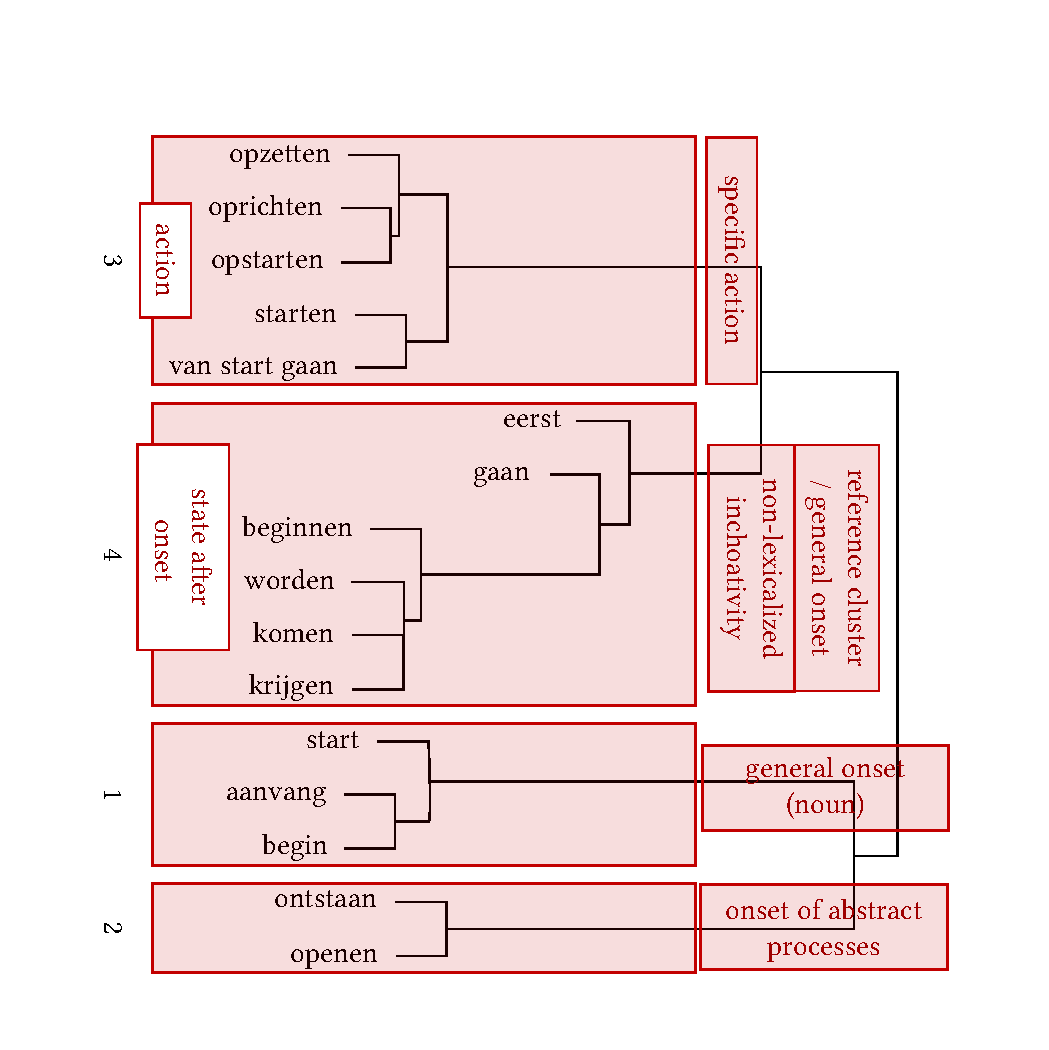
\includegraphics[width=.75\textwidth,trim=0 20 0 50]{figures/tree86.pdf}
\caption{\label{fig:4:83}Dendrogram representing a semantic field of \textit{beginnen}/inchoativity for TransDutch\textsubscript{FR} with meta-labels.}
\end{figure}

In conclusion, the following similarities have been observed for the three visualizations: For all three visualizations, the cluster closest to the zero-point of the semantic space (considered as the prototypical center) was indicated as the \textsc{reference cluster}. In addition, the initial lexeme \textit{beginnen} is part of the \textsc{reference cluster} in all three visualizations.\textsubscript{} Since \textit{beginnen} is considered as the most prototypical expression of inchoativity, I believe that the \textsc{reference cluster}\textit{/}\textsc{general onset} contains the most prototypical expressions of inchoativity. 

For all three visualizations, the distance of the lexemes in the \textsc{reference cluster} to the abstract prototypes of the other clusters is fairly equal. This implies that the \textsc{reference cluster} is indeed the most central one in the semantic space and shows the least deviation with respect to the other clusters (the lexemes in the \textsc{reference cluster} are all fairly equally similar to the abstract prototypes of the other clusters). Furthermore, the semantic proximity of cluster n°4 to the \textsc{reference cluster} in TransDutch\textsubscript{ENG} is confirmed by the similar distance of the lexemes in both clusters to the abstract prototypes of other clusters. For TransDutch\textsubscript{FR}, the semantic proximity between the cluster containing {\textsc{specific}} \textsc{action} and \textsc{action} to the \textsc{reference cluster} is also confirmed by the equal distances of the lexemes of both clusters to the abstract prototypes of the other clusters. In all three visualizations, nouns and verbs are clustered separately. However, it cannot be maintained that clustering is totally independent of word class, since in the TransDutch fields, \textit{eerst} becomes part of the \textsc{reference cluster} and clusters with lexemes of a distinct word class.

\section{Levelling out}
\label{sec:4.5}  
In \sectref{sec:4.2}, \sectref{sec:4.3} and \sectref{sec:4.4} I formulated a number of insights with respect to the proto\-type-based organization of the clusters and the lexemes in each of the fields of SourceDutch, TransDutch\textsubscript{ENG} and TransDutch\textsubscript{FR} on the basis of centroids and medoids. These insights will now be used to see whether translation has impacted the organization of the fields on the semasiological or the onomasiological level and whether or not levelling out has taken place.

On the semasiological level, I will assess the changes in the distances of the clusters’ centroids to the zero-point of the semantic space (considered as the prototypical center) they belong to amongst the different varieties. If the prototype-based organization of those meanings in translated Dutch differs from that in non-translated Dutch, and if this difference furthermore consists in \textit{beginnen} having fewer different meaning differentiations in translated language compared to \textit{beginnen} in non-translated Dutch, I will call the phenomenon semasiological levelling out.

On the onomasiological level, I will assess the changes in the distances of the lexemes in each cluster to the centroid (the abstract prototype) of the cluster they belong to. I will investigate whether the prototype-based organization of the lexemes in each cluster (with each cluster expressing a particular meaning differentiation) in translated Dutch differs from that in non-translated Dutch. My method does however not allow me to investigate whether a given concept is expressed by fewer lexemes in translated Dutch compared to the same concept in non-translated Dutch, because the total number of lexemes within each semantic field is kept stable over all visualizations (see \sectref{sec:3.5.3}).\footnote{Since the number of lexemes is kept stable, any concept expressed by fewer lexemes would necessarily lead to another concept being expressed by more lexemes.} Observations on the onomasiological level will inform me about differences in the prototype-based organization of each cluster and possible changes in near-synonymy relationships between the lexemes in the semantic field under the influence of translation.

I first give a schematic overview of the observations on both the semasiological and the onomasiological level. The changes between the field of SourceDutch on the one hand and the fields of TransDutch\textsubscript{ENG} and TransDutch\textsubscript{FR} will be described subsequently.

\begin{sidewaystable}
\caption{SourceDutch}
\scriptsize
\begin{tabularx}{\textwidth}{cp{3.6cm}p{2.4cm}p{5.4cm}X}
\lsptoprule
Cl. & Meta-label(s) & Lexemes in cluster & Semasiological phenomena & Onomasiological phenomena \\\midrule 
\rowcolor{lsLightGray} 3 & \textsc{reference cluster} / \newline \textsc{general onset} & \itshape opstarten\newline starten\newline van start gaan\newline beginnen\newline gaan & closest to prototypical center;\newline \textsc{action};\newline \textsc{state after onset} & competition between \textit{beginnen} and \textit{starten} for position closest to the abstract prototype\\
2 & \textsc{general onset} (\textsc{noun}) & \itshape start\newline aanvang\newline begin & second closest to prototypical center; \newline closest to \textsc{reference cluster} &  competition between \textit{start} and \textit{begin} for position closest to the abstract prototype\\
\rowcolor{lsLightGray} 1 & \textsc{specific} \textsc{action} & \itshape oprichten\newline opzetten &  & \\
5 & \textsc{non-lexicalized} \newline \textsc{inchoactivtiy} & \itshape komen\newline krijgen\newline worden &  & \\
\rowcolor{lsLightGray} 4 & \textsc{onset of abstract}\newline \textsc{processes} & \itshape ontstaan\newline openen &  & \\
6 &  & \itshape eerst &  & \\
\lspbottomrule
\end{tabularx}
\normalsize
\end{sidewaystable}

\begin{sidewaystable}
\caption{TransDutch\textsubscript{ENG}}
\scriptsize
\begin{tabularx}{\textwidth}{cp{3.6cm}p{2.4cm}p{5.3cm}X}
\lsptoprule
Cl. & Meta-label(s) & Lexemes in cluster & Semasiological phenomena and changes & Onomasiological phenomena and changes\\\midrule 
\rowcolor{lsLightGray} 3 & \textsc{reference cluster} / \newline \textsc{general onset} & \itshape eerst\newline van start gaan\newline beginnen\newline krijgen\newline starten\newline gaan\newline worden & closest to prototypical center;\newline  +\textit{eerst};\newline +\textsc{non-lexicalized inchoativity};\newline \textsc{action} vs.\ \textsc{state after onset} unclear & \textit{beginnen} closest to abstract prototype ($<$ SourceDutch $<$ TransDutch\textsubscript{FR});\newline  more lexemes ($\leftrightarrow $ SourceDutch);\newline  distance to abstract prototype: \textit{beginnen} $<$ \textit{gaan} $<$ \textit{krijgen} $<$ \textit{worden} $<$ \textit{starten} $<$ \textit{van start gaan} \\
4 & \textsc{no label} & \itshape komen\newline opstarten & second closest to prototypical center & \\
\rowcolor{lsLightGray} 2 & \textsc{onset} (\textsc{noun}) & \itshape begin &  & \textit{begin} closest to abstract prototype ($<$ SourceDutch $<$ TransDutch\textsubscript{FR})\\
6 & \textsc{onset} (\textsc{noun}) & \itshape aanvang\newline start & closer to prototypical center than cluster 2 & larger difference in distance to abstract prototype between \textit{aanvang} and \textit{start} ($\leftrightarrow$ SourceDutch)\\
\rowcolor{lsLightGray} 1 & \textsc{specific} \textsc{action} & \itshape oprichten\newline opzetten &  & larger difference in distance to abstract prototype between \textit{oprichten} and \textit{opzetten} ($\leftrightarrow $ SourceDutch)\\
5 & \textsc{onset of abstract} \newline \textsc{processes} & \itshape ontstaan\newline openen &  & smaller difference in distance to abstract prototype between \textit{openen} and \textit{ontstaan} ($\leftrightarrow $ SourceDutch)\\
\lspbottomrule
\end{tabularx}
\normalsize
\end{sidewaystable}

\begin{sidewaystable}
\caption{TransDutch\textsubscript{FR}}
\scriptsize
\begin{tabularx}{\textwidth}{cp{3.6cm}p{2.4cm}p{5.3cm}X}
\lsptoprule

Cl. & Meta-label(s) & Lexemes in cluster & Semasiological phenomena and changes & Onomasiological phenomena and changes\\
\midrule 
\rowcolor{lsLightGray} 4 & \textsc{reference cluster} & \itshape eerst\newline gaan\newline beginnen\newline worden\newline komen\newline krijgen & closest to prototypical center;\newline  + \textit{eerst};\newline  +\textsc{non-lexicalized inchoativity};\newline \textsc{state after onset} & 
\textit{beginnen} furthest away from abstract prototype ($>$ SourceDutch $>$ TransDutch\textsubscript{ENG});\newline  more lexemes $\leftrightarrow $ SourceDutch\\
3 & \textsc{specific} \textsc{action} & \itshape opzetten\newline oprichten\newline opstarten\newline starten\newline van start gaan &  second closest to prototypical center;\newline  \textsc{action} & +\textit{opstarten};\newline larger difference in distance to abstract prototype between \textit{oprichten} and \textit{opzetten} ($\leftrightarrow $ SourceDutch)\\
\rowcolor{lsLightGray} 1 & ONSET (\textsc{noun}) & \itshape begin\newline aanvang\newline gaan &  & distance to prototype: \textit{begin} $<$ \textit{aanvang} $<$ \textit{start}\\
2 &\textsc{onset of abstract processes} & \itshape ontstaan\newline openen &  & smaller difference in distance to prototype between \textit{openen} and \textit{ontstaan} ($\leftrightarrow $ SourceDutch);\newline distance to prototype: \textit{ontstaan} $<$ \textit{openen}\\
\lspbottomrule
\end{tabularx}
\normalsize
\end{sidewaystable}

\clearpage

\subsection{\label{sec:4.5.1}Semasiological levelling out}

On the semasiological level, I observe the following changes for the \textsc{reference cluster}\slash\textsc{general onset} (\figref{fig:4:84}):


\begin{itemize}
\item  In TransDutch\textsubscript{ENG}, the \textsc{reference cluster} contains the meaning distinctions \textit{eerst} and {\textsc{non-lexicalized inchoativity}} in addition to \textsc{general onset} (the only meta-label for this cluster in SourceDutch). The distinction between \textsc{action} and \textsc{state after onset} remains unclear on the semasiological level for TransDutch\textsubscript{ENG}.
\item  In TransDutch\textsubscript{FR}, the \textsc{reference cluster} contains the meaning distinctions \textit{eerst} and {\textsc{non-lexicalized inchoativity}} in addition to \textsc{general onset} (the only meta-label for this cluster in SourceDutch). It does not, however, contain the meaning distinction \textsc{action}.
\item  In both TransDutch visualizations, more meaning distinctions become part of the \textsc{reference cluster} compared to SourceDutch. In both TransDutch fields, the meaning distinctions \textit{eerst} and {\textsc{non-lexicalized inchoativity}} become part of the \textsc{reference cluster}, implying that they are used more prominently in TransDutch compared to SourceDutch.
\end{itemize}

\begin{figure}
% 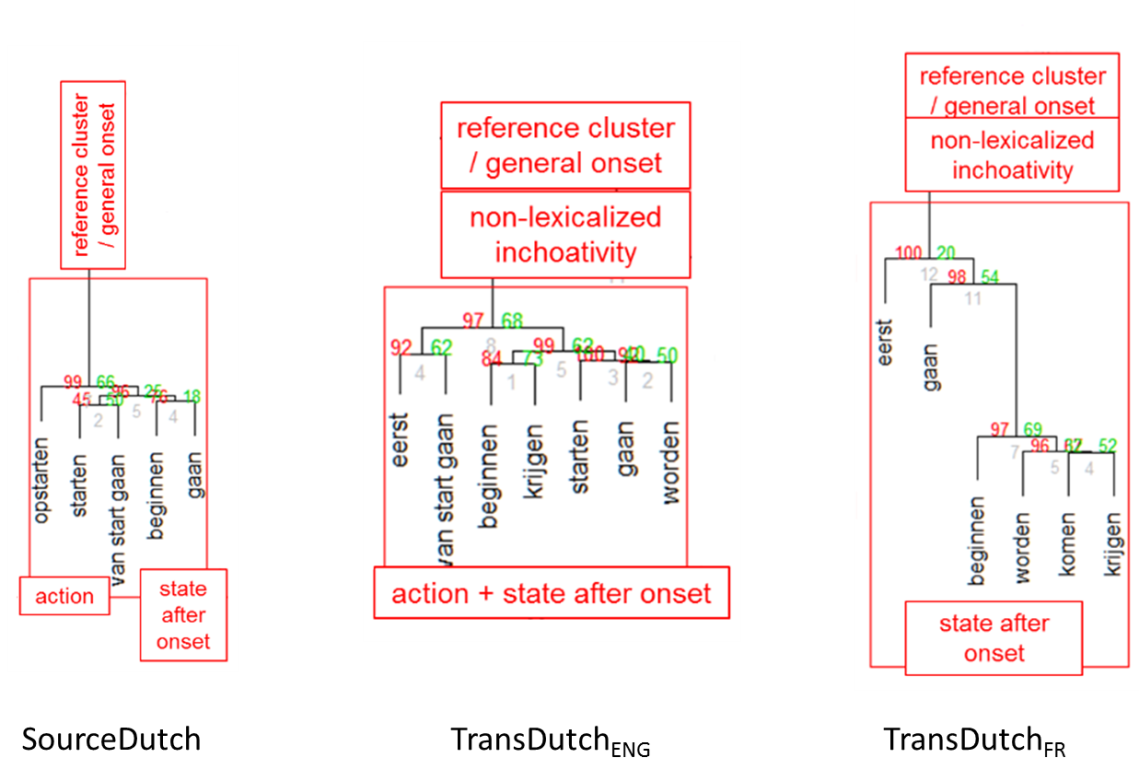
\includegraphics[height=.4\textheight]{figures/Vandevoorde2-img87.png}
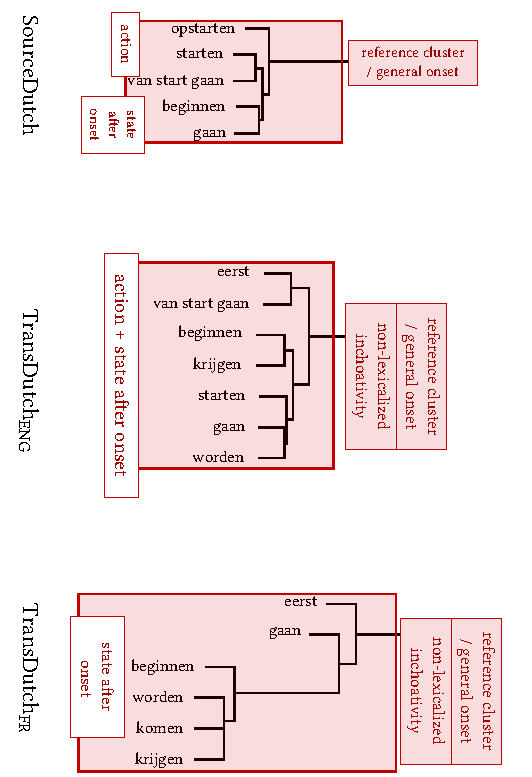
\includegraphics{figures/tree87.pdf}
\caption{\label{fig:4:84}\textsc{reference cluster}/\textsc{general onset} of SourceDutch, TransDutch\textsubscript{ENG} and TransDutch\textsubscript{FR}}
\end{figure}

\noindent For \textsc{general onset} (\textsc{noun}) (\figref{fig:4:85}), the following observations can be made:

\begin{itemize}
\item  In TransDutch\textsubscript{ENG}, \textit{begin} forms a distinct cluster, whereas in SourceDutch, \textit{begin} was part of \textsc{general onset} (\textsc{noun}). This division on the semasiological level suggests an additional meaning distinction within \textsc{general onset} (\textsc{noun}) in TransDutch\textsubscript{ENG}.
\end{itemize}

\begin{figure}[p]
% 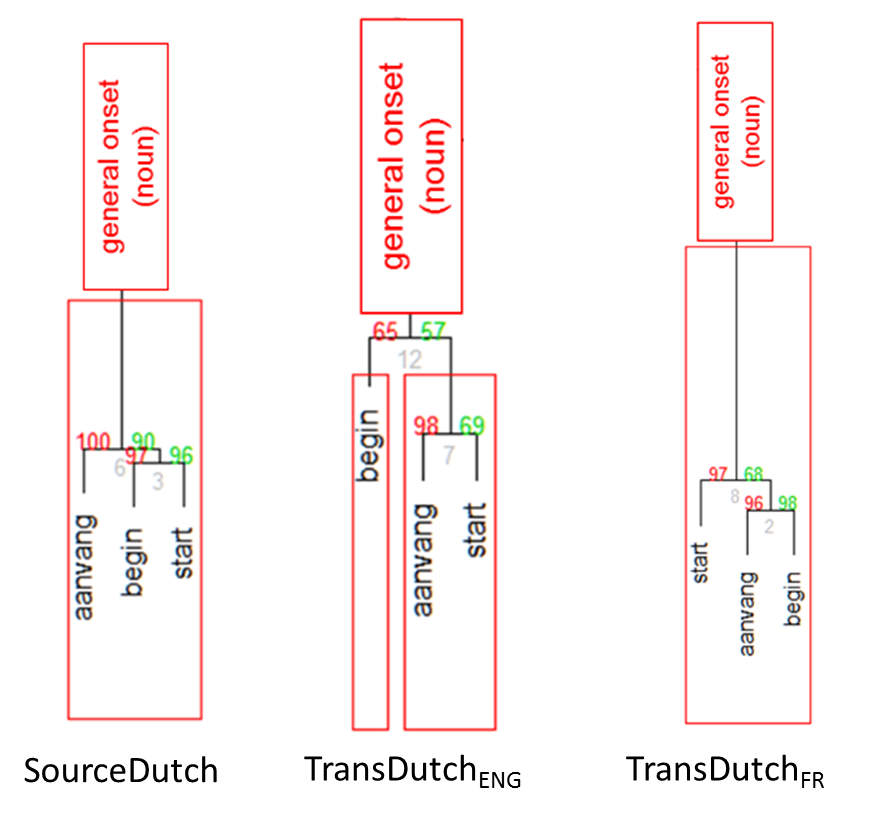
\includegraphics[height=.4\textheight]{figures/Vandevoorde2-img88.png}
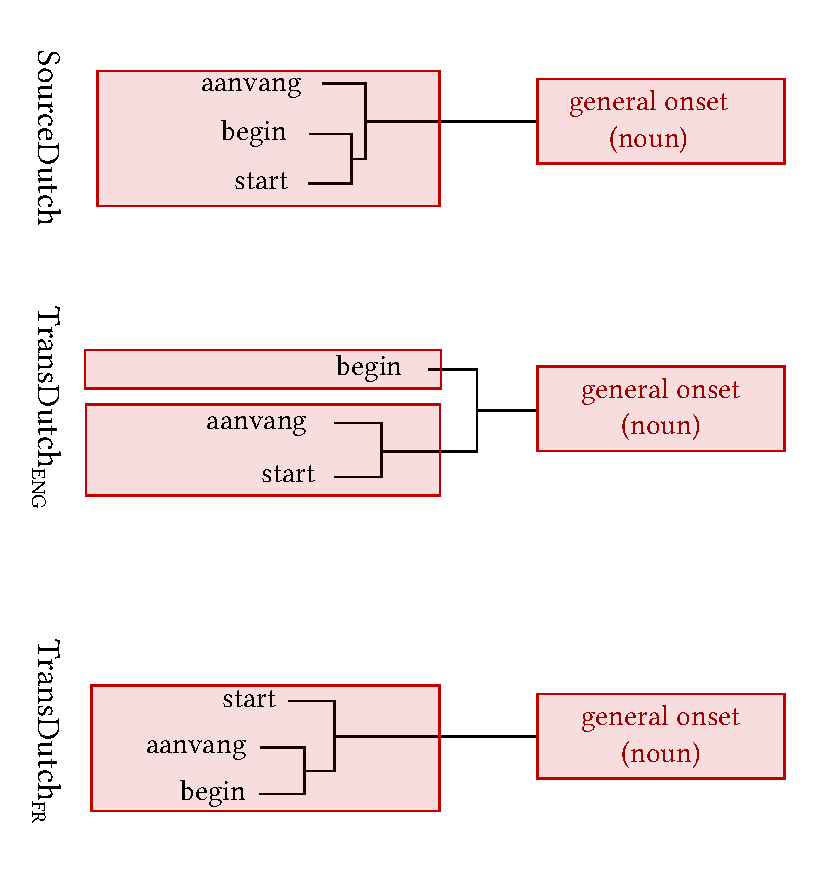
\includegraphics[width=9cm]{figures/tree88.pdf}
\caption{\label{fig:4:85}\textsc{general onset (noun)} of SourceDutch, TransDutch\textsubscript{ENG} and TransDutch\textsubscript{FR}}
\end{figure}

\begin{figure}[p]
% 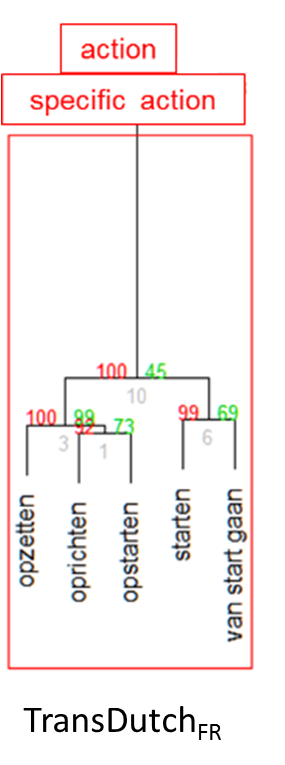
\includegraphics[height=.4\textheight]{figures/Vandevoorde2-img89.png}
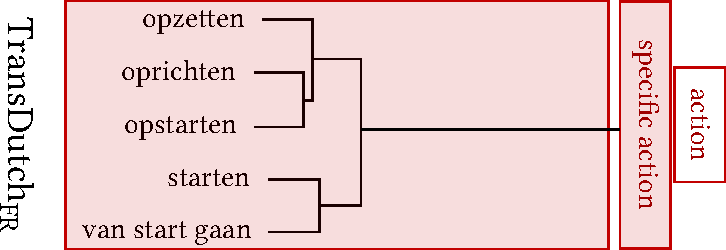
\includegraphics[width=7cm]{figures/tree89.pdf}
\caption{\label{fig:4:86}\textsc{action}/\textsc{specific} \textsc{action} for TransDutch\textsubscript{FR}}
\end{figure}

\noindent For \textsc{action} (\figref{fig:4:86}), my observations are as follows:

\begin{itemize}
\item  In TransDutch\textsubscript{FR}, a cluster is formed containing \textsc{action} and {\textsc{specific}} \textsc{action}. This new cluster (meaning distinction) emphasizes the dynamic nature (the common denominator of \textsc{action} and {\textsc{specific}} \textsc{action}) of the verbs it contains. In addition, the distinction between \textsc{action} and \textsc{state after onset} becomes more clearly marked in TransDutch\textsubscript{FR}, compared to both SourceDutch and TransDutch\textsubscript{ENG} since \textsc{action} and \textsc{state after onset} now pertain to separate clusters.
\end{itemize}

From a semasiological point of view, it can be concluded that in translation, the meaning distinctions revealed by the different clusters do indeed differ from those in SourceDutch. In both TransDutch fields, some of the meaning distinctions that had been discerned for SourceDutch are now conflated in the \textsc{reference cluster}. The cluster of \textsc{general onset} in both TransDutch fields thus ``absorbs'' a certain amount of the semasiological variation that was present in SourceDutch. Fewer of the meanings that were distinguished in SourceDutch are distinguished in the TransDutch fields. As a consequence, a presence of semantic levelling out on the semasiological level can be claimed here. Two observations seem however to go against this statement. First, for TransDutch\textsubscript{FR}, on the one hand, the meaning distinction between \textsc{action} and \textsc{state after onset} is emphasized compared to SourceDutch (\textsc{action} and \textsc{state after onset} are now part of two distinct clusters, implying no levelling out), while on the other hand, the conflation of \textsc{action} and {\textsc{specific}} \textsc{action} erases the meaning distinction between \textsc{action} and {\textsc{specific}} \textsc{action}, so that levelling out on the semasiological level can be claimed. Second, in TransDutch\textsubscript{ENG}, a meaning distinction containing only \textit{begin} is suggested, and a second one containing \textit{opstarten} and \textit{komen} is also discerned, implying more semasiological specification than in SourceDutch.

\subsection{Onomasiological changes in the prototype-based organization}
\label{sec:4.5.2}  
On the onomasiological level, the following changes can be observed for the \textsc{reference cluster}\textit{/}\textsc{general onset}. The unclear distinction between \textsc{action} and \textsc{state after onset} in TransDutch\textsubscript{ENG} is clarified on the onomasiological level: the distances of the lexemes to the abstract prototype (centroid) of the \textsc{reference cluster} of TransDutch\textsubscript{ENG} show that \textsc{state after onset} verbs (\textit{beginnen} and \textit{gaan}) are closer to the abstract prototype, but that \textsc{action} verbs (\textit{starten} and \textit{van start gaan}) are situated much further away from the abstract prototype. This organization is different from SourceDutch, where \textit{beginnen} and \textit{starten} are both at a minimal distance to the abstract prototype. In other words, the difference in distance to the prototype between \textit{starten} and \textit{beginnen} becomes larger in TransDutch\textsubscript{ENG}, compared to SourceDutch. In TransDutch\textsubscript{FR}, \textit{starten} and \textit{beginnen} are part of different clusters (and hence more dissimilar). For both TransDutch semantic representations, \textit{beginnen} and \textit{starten} are less near-synonymous than in SourceDutch.

In \textsc{general onset} (\textsc{noun}), \textit{start} and \textit{begin} compete for the position closest to the abstract prototype in SourceDutch. In both TransDutch fields, the competition between \textit{begin} and \textit{start} is less present: in TransDutch\textsubscript{ENG}, a separate cluster with \textit{begin} appears, and in TransDutch\textsubscript{FR}, \textit{begin} is closest to the abstract prototype, but \textit{start} is situated much further away from the abstract prototype. \textit{Begin} and \textit{start} are thus less near-synonymous in both TransDutch\textsubscript{} fields compared to SourceDutch.

In {\textsc{specific}} \textsc{action}, a competition for the position closest to the abstract prototype is also going on between \textit{oprichten} and \textit{opzetten}. A similar situation appears here: in SourceDutch, both lexemes are extremely close to the abstract prototype, whereas in the TransDutch fields, the difference in distance to the abstract prototype increases, implying that the lexemes are less near-synonymous in TransDutch compared to SourceDutch.

From an onomasiological point of view, a number of small differences in the prototype-based organization of the lexemes are observed in TransDutch compared to SourceDutch. S\textit{tarten} and \textit{beginnen} become less near-synonymous (the difference in distance between the lexemes with respect to the prototype becomes larger) in both TransDutch fields. The same observation can be made for \textit{start} and \textit{begin}: the two lexemes are more near-synonymous in SourceDutch, but less near-synonymous in TransDutch\textsubscript{ENG} and TransDutch\textsubscript{FR}. This is also observed for \textit{oprichten} and \textit{opzetten}: they are more synonymous in SourceDutch compared to TransDutch\textsubscript{ENG} and TransDutch\textsubscript{FR}. Although the joint clustering of (pairs of) lexemes of course confirms the synonymy between the lexemes, it could be concluded that lexemes which are near-synonyms in SourceDutch (such as \textit{starten} and \textit{beginnen}, \textit{start} and \textit{begin}, \textit{oprichten} and \textit{opzetten}) tend to become less near-synonymous in translated language. Note that this trend has only been observed for lexemes which are near-synonyms in SourceDutch (both very close to the abstract prototype). For lexemes pertaining to the same cluster (which can also be considered as synonyms given their joint clustering) which show larger differences in distance to the prototype in SourceDutch (indicating less near-synonymy) such as \textit{ontstaan} and \textit{openen}, the difference in distance to the abstract prototype is not increased by translation.

\section{Shining through}\label{sec:4.6}  
\subsection{Semasiological shining through}\label{sec:4.6.1}  
Semasiological shining through (source language influence on the meaning distinctions in translated language) is investigated by comparing the meaning distinctions in translated language to those present in the source language of the translation. To do so, the semantic fields of the closest equivalents of \textit{beginnen} in the source languages of TransDutch\textsubscript{ENG} and TransDutch\textsubscript{FR} are visualized: SourceEnglish \textit{to begin} and SourceFrench \textit{commencer}.

Ideally, I should first provide an analysis of SourceEnglish and SourceFrench following the exact same steps as for SourceDutch (a statistical visualization, followed by a description of the prototype-based organization of the semantic field on both the semasiological and the onomasiological level, leading to an in depth description and interpretation of the semantic field) before comparing the different meaning distinctions (clusters) in the fields of \textit{to begin} and \textit{commencer} to the meaning distinctions in TransDutch\textsubscript{ENG} and TransDutch\textsubscript{FR}. I will however only present the visual output of the HAC (carried out on the output of a CA, according to the exact same procedure as described in \chapref{sec:3}) for SourceEnglish and SourceFrench without providing a lengthy discussion of the prototype-based organization of those two fields. A full description – the ideal scenario – would require a complete contrastive comparison of the fields of SourceEnglish and SourceFrench (and SourceDutch) before the influence of SourceEnglish and SourceFrench on TransDutch\textsubscript{ENG} and TransDutch\textsubscript{FR} could be determined. Obviously, such a description would enhance the insights into the influence on the target language of attested differences between the source language and the target language semantic fields. I will, however, present the visualizations of SourceEnglish and SourceFrench in the light of the possible explanations they could provide for a number of differences observed in the TransDutch\textsubscript{ENG} and TransDutch\textsubscript{FR} fields and which are possibly caused by specific source language influence.

\subsubsection{Semasiological shining through of SourceEnglish}
\label{sec:4.6.1.1}  
Three semasiological changes in TransDutch\textsubscript{ENG} (compared to SourceDutch) might have been influenced by existing meaning distinctions in SourceEnglish: (i) the separate clustering of \textit{begin}, (ii) the separate clustering of \textit{opstarten} and \textit{komen}\footnote{Since the clustering of \textit{komen} is unstable (\sectref{sec:4.3.1}), the analysis will mainly focus on \textit{opstarten}.} and (iii) the unclear distinction between \textsc{action} and \textsc{state after onset} (on the semasiological level) in the \textsc{reference cluster} of TransDutch\textsubscript{ENG}. A source language influence could be claimed if, in SourceEnglish, a separate meaning distinction (cluster) containing the closest translational equivalent of \textit{begin}, i.e. \textit{beginning} was attested and\slash or a separate meaning distinction containing \textit{to start up} and \textit{to come} (the closest translational equivalents of \textit{opstarten} and \textit{komen}). If in SourceEnglish, the meaning distinction (possibly within the most central cluster of the analysis) between \textsc{action} and \textsc{state after onset} is equally unclear as in TransDutch\textsubscript{ENG}, this could possibly be interpreted this as source language influence.

The semantic field of SourceEnglish was visualized on the basis of data retrieved via the SMM++ with \textit{to begin} as initial lexeme and Dutch as a Language B. The exact same procedure as for SourceDutch was followed. One important difference needs to be noted here: since the DPC does not contain data for the translation directions French to English and English to French, only one language can be used as a Language B when an English initial lexeme is chosen, in casu, Dutch. The establishment of the data set for SourceEnglish was consequently only based on the second T-image of \textit{to begin} with Dutch as a pivot language (recall that for SourceDutch, the data sets of the second T-image of \textit{beginnen}\textsubscript{FR} and \textit{beginnen}\textsubscript{ENG} were combined).\footnote{One could argue here that the semantic field of SourceEnglish is likely to be biased by the fact that the used data set is only based on the second T-image of \textit{to begin} with Dutch as a source language. In order to solve this problem while maintaining our translational method, I would have needed a tri-directional corpus (where all three languages can be used as languages B to carry out a SMM++) which I do not have at my disposal. Another solution would have been to apply an alternative, distributional technique to visualize the SourceLanguage semantic fields which would only use monolingual (Dutch) data to create the data matrix (rather than the translations). A comparison of the translational and the distributional approach is provided in \citet{vandevoorde_distributional_2016} and shows that the patterns revealed by both methods are very similar.} The outcome of the SMM++ retrieval task rendered a set of 30 English lexemes (911 observations). I carried out a HAC on the output of the CA and chose a cluster solution with 5 clusters (average silhouette width 0.7).

\begin{figure}
% 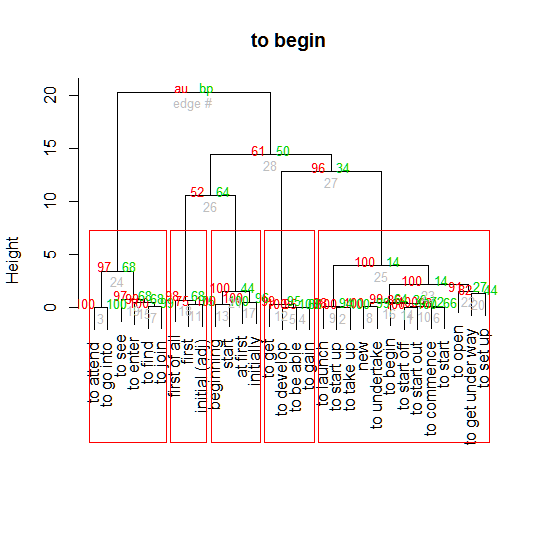
\includegraphics[height=.4\textheight]{figures/Vandevoorde2-img90.png}
\includegraphics[width=.75\textwidth,trim=0 20 0 50]{figures/tree90.pdf}
\caption{\label{fig:4:87}Dendrogram representing a semantic field of \textit{to begin} for SourceEnglish}
\end{figure}

The dendrogram (\figref{fig:4:87}) for SourceEnglish shows that \textit{beginning} is part of a cluster with \textit{start}, \textit{at first} and \textit{initially} so that no separate meaning distinction of \textit{beginning} is implied by SourceEnglish. Consequently, the separate meaning distinction of \textit{begin} in TransDutch\textsubscript{ENG} could not have been triggered by an existing meaning distinction in SourceEnglish.

The verb \textit{to start up} is part of the largest cluster (and the most central one in the semantic space) of the analysis, containing both \textit{to start} and \textit{to begin}. The closest translational equivalent of \textit{komen}, \textit{to come} is not a lexeme in the SourceEnglish visualization.\footnote{\textit{Komen} is a verb which typically does not lexicalize inchoativity and draws its inchoative meaning from the context it is used in. As a consequence, its closest translational equivalent \textit{to come} does not typically express inchoativity and is, unsurprisingly, not a member of the SourceEnglish field.} On the basis of this information, I conclude that the separate meaning distinction of \textit{komen} and \textit{opstarten} in TransDutch\textsubscript{ENG} is not caused by an existing meaning distinction in SourceEnglish.

As for the unclear distinction between \textsc{action} and \textsc{state after onset} in TransDutch\textsubscript{ENG}, no clear division between \textsc{action} and \textsc{state after onset} is marked in SourceEnglish either. The prototypical \textsc{action} verb \textit{to start} and the prototypical \textsc{state after onset} verb \textit{to begin} are both part of the same, most central cluster (the outer right cluster in the dendrogram), although they belong to different sub-nodes (just as was the case for TransDutch\textsubscript{ENG} and SourceDutch). Semasiological shining through could be claimed here, although it must be admitted that -- given the similar divide between \textsc{action} and \textsc{state after onset} in SourceDutch – the phenomenon could well be interpreted as semasiological normalization too (see \sectref{sec:4.7.1}).

\subsubsection{Semasiological shining through of SourceFrench}
\label{sec:4.6.1.2}  
For TransDutch\textsubscript{FR,} the meaning distinctions \textsc{action} and {\textsc{specific}} \textsc{action} are ``absorbed'' by a new cluster. This new cluster emphasizes the (common) dynamic nature of the meaning distinctions it absorbed (while the specificity of the meaning distinctions indicated by \textsc{action} and {\textsc{specific}} \textsc{action} is somewhat ``levelled out''). In addition, the distinction between \textsc{action} and \textsc{state after onset} is more emphasized in TransDutch\textsubscript{FR} (the labels are assigned to different clusters), compared to SourceDutch and SourceEnglish (where \textsc{action} and \textsc{state after onset} pertain to the \textsc{reference cluster}). In this section, I will now investigate whether source language influence has possibly caused this semasiological change.

The data for the visualization of SourceFrench were retrieved via the SMM++ with \textit{commencer} as initial lexeme and Dutch as Language B. Parallel to the field of SourceEnglish, the field of SourceFrench (\figref{fig:4:88}) is only based on data from the second T-image of \textit{commencer} with Dutch as Language B. The SMM++ retrieval task rendered a set of 25 French lexemes (824 observations). I carried out a HAC on the output of the CA. The chosen cluster solution with 4 clusters obtained an average silhouette width of 0.54.

\begin{figure}
% \includegraphics[height=.4\textheight]{figures/Vandevoorde2-img91.png}
\includegraphics[width=.75\textwidth,trim=0 20 0 50]{figures/tree91.pdf}
\caption{\label{fig:4:88}Dendrogram representing a semantic field of \textit{commencer} for SourceFrench}
\end{figure}

Like in English (and Dutch), inchoativity in French is also thought to present the division between more dynamic \textsc{action} verbs (“focusing on the transition from \textsc{non-action} to \textsc{action}”) and more static \textsc{state after onset} verbs (“indicating the start of a transformation”) \citep[241]{vogeleer_linchoatif:_1999}. Although Marque-Pucheu does not specify any particular verbs of inchoativity that are more typically used with the one rather than with the other verb type, clearly, \textit{démarrer} `to start up', \textit{entamer} `to start' and \textit{débuter} `to begin, to start' are verbs that can be categorized as \textsc{action} verbs (they are used with \textit{moteur} `engine' for example), while \textit{commencer} (the translational equivalent of \textit{to begin}) seems to focus on the \textsc{state after onset}. Within SourceFrench, there is indeed a cluster containing these \textsc{action} verbs \textit{entamer}, \textit{débuter}, \textit{démarrer}, \textit{au départ} `initially' and \textit{lancer} `to launch'. Within the cluster containing \textit{commencer}, some of the lexemes indeed suggest that this cluster is focusing on the more static \textsc{state after onset}. \textit{Entrer}, for instance, can indicate \textit{commencer à être dans un lieu, à un endroit, dans un état}, \textit{dans une période} `to start being in a place, state, period…' (\textit{Grand Robert de La Langue Française}, 2013), and \textit{se mettre}, can mean \textit{devenir quant à l'état physique, la situation} `to become into a physical state, a situation' or -- when followed by the preposition \textit{à} – \textit{commencer à faire} `to begin to do something'. It could be claimed that in SourceFrench, a clear meaning distinction is made between \textsc{action} and \textsc{state after onset} (they make up distinct clusters). The separate clustering of \textsc{action} and \textsc{state after onset} in TransDutch\textsubscript{FR} might then have been triggered by the distinct clustering of \textsc{action} and \textsc{state after onset} in SourceFrench as an instance of semasiological shining through.

However, in the same cluster of \textit{commencer}, there are also a number of lexemes present which seem to be more related to business-like contexts (and could easily be labelled as {\textsc{specific}} \textsc{action}), such as \textit{entreprendre} `to undertake' and \textit{se lancer} `to launch oneself into'. These lexemes expressing {\textsc{specific}} \textsc{action} are clustering with \textsc{state after onset} in SourceFrench, whereas in TransDutch\textsubscript{FR}, they form a cluster with \textsc{action}. As a consequence, the joint clustering of \textsc{action} and {\textsc{specific}} \textsc{action} cannot be explained on the basis of semasiological shining through.

The above interpretation is of course preliminary, and can only hint towards possible instances of semasiological shining through. A more thorough analysis of the SourceEnglish and the SourceFrench field is needed to understand the mechanisms of source language influence on the TransDutch fields. For TransDutch\textsubscript{FR}, for example, such an analysis would have to confirm or disaffirm whether the presumed distinction between \textsc{action} and \textsc{state after onset} does indeed correspond to the lexemes in the respective clusters of SourceFrench and\slash or whether the assumed joint clustering of {\textsc{specific}} \textsc{action} with \textsc{state after onset} in SourceFrench can indeed be claimed.

\subsection{Onomasiological shining through}
\label{sec:4.6.2}  
Two additional visualizations for TransDutch\textsubscript{ENG} and TransDutch\textsubscript{FR} are presented in this section, containing the English and French source language lexemes together with the Dutch target language lexemes. In this way, onomasiological shining through can be investigated. In other words, it can be determined whether the organization of the lexical items in the meaning distinctions in the fields of TransDutch\textsubscript{ENG} and TransDutch\textsubscript{FR} is influenced by a specific underlying source language lexeme. Rather than describing the influence of each underlying English or French source language lexeme, I will focus on those instances where a specific source language lexeme might explain a change in the organization of the lexemes in TransDutch\textsubscript{ENG} or TransDutch\textsubscript{FR} compared to SourceDutch.


\subsubsection{Onomasiological shining through of English}
\label{sec:4.6.2.1}  
In \sectref{sec:4.6.1}, I concluded that semasiological shining through could not account for the separate clustering of \textit{begin}, nor for the separate clustering of \textit{opstarten} in TransDutch\textsubscript{ENG}. I will now explore whether this separate clustering could be the result of an instance of onomasiological shining through (the influence of a specific source language lexeme).

The simultaneous visualization of the source and target language lexemes in a single space is carried out via a Multiple Correspondence Analysis on a Burt Table \citep{greenacre_simple_2006, greenacre_correspondence_2007} (see \sectref{sec:3.8}). I use the output of the Multiple Correspondence Analysis, as the input for a HAC. Although the visualization of the HAC on the output of a MCA at first sight looks quite different from the dendrogram representing a semantic field of \textit{beginnen} for TransDutch\textsubscript{ENG}, the two visualizations do depict the same reality: the clustering of the Dutch lexemes in \figref{fig:4:89}\footnote{The clusters are numbered from left to right.} below is identical to that in \figref{fig:4:64} (all clusters correspond to either a cluster or a sub-node).\footnote{Note that the lexemes from cluster n°4 from TransDutch\textsubscript{ENG} (\textit{komen} and \textit{opstarten}) are now spread over two different clusters – this was to be expected given the ``unstable'' clustering in TransDutch\textsubscript{ENG} of those two lexemes. The lexemes of the \textsc{reference cluster} of TransDutch\textsubscript{ENG} (cluster n°3) are now spread over two clusters, which are joined in a higher, slightly less significant node within this visualization.}

\begin{figure}
% \includegraphics[height=.4\textheight]{figures/Vandevoorde2-img92.png}
\includegraphics[width=.75\textwidth,trim=0 20 0 50]{figures/tree92.pdf}
\caption{\label{fig:4:89}Representation of HAC on the MCA for TransDutch\textsubscript{ENG}}
\end{figure}

On a general level, it is striking that all English source language lexemes are clustered together with their Dutch close cognate whenever the latter is present in the analysis (only \textit{first of all} and \textit{to start out} do not have direct close cognate amongst the Dutch lexemes). I discern the following pairs: \textit{beginning} -- \textit{begin}; \textit{start} -- \textit{start}; \textit{to open} -- \textit{openen}; \textit{to begin} -- \textit{beginnen}; \textit{to start} -- \textit{starten}; \textit{to start up} -- \textit{opstarten}; \textit{to set up} -- \textit{opzetten}.

Dutch \textit{begin} is clustered with its English close cognate \textit{beginning} (cluster n°6), revealing the preference of \textit{begin} to be used as a translation of \textit{beginning}. The same goes for \textit{opstarten}, which is clustered here with its close cognate \textit{to start up}. In both cases, the underlying English source language lexemes seem to trigger the separate clustering of \textit{begin} and \textit{opstarten}. In this way, an influence on the onomasiological level seems to provoke semasiological change in TransDutch\textsubscript{ENG} compared to SourceDutch. This onomasiological shining through is very likely to be triggered by the strong semantic relatedness between the elements of pairs of close cognates such as \textit{begin} -- \textit{beginning} and \textit{opstarten} -- \textit{to start up.}

\subsubsection{Onomasiological shining through of French}
\label{sec:4.6.2.2}  
In \sectref{sec:4.6.1.2}, I tentatively accounted for the clear (over-emphasized with respect to SourceDutch) meaning distinction between \textsc{action} and \textsc{state after onset} in TransDutch\textsubscript{FR} via semasiological shining through. The joint clustering of \textsc{action} and {\textsc{specific}} \textsc{action} could however not be explained on the semasiological level. In this section, I want to investigate whether the joint clustering of \textsc{action} and {\textsc{specific}} \textsc{action} could be the result of an instance of onomasiological shining through (the influence of a specific source language lexeme on the organization of the lexemes within a cluster\slash meaning distinction).

The clustering of the Dutch lexemes presented in the visualization in \figref{fig:4:90}\footnote{The clusters are numbered from left to right.} shows the same semantic field of \textit{beginnen} for TransDutch\textsubscript{FR} as the dendrogram of the HAC for TransDutch\textsubscript{FR} in \figref{fig:4:76} (all clusters correspond to either a cluster or a sub-node).

\begin{figure}
% \includegraphics[height=.4\textheight]{figures/Vandevoorde2-img93.png}
\includegraphics[width=.75\textwidth,trim=0 20 0 50]{figures/tree93.pdf}
\caption{\label{fig:4:90}Representation of HAC on the MCA for TransDutch\textsubscript{FR}}
\end{figure}

The cluster reuniting {\textsc{specific}} \textsc{action} and \textsc{action} in the HAC visualization in \figref{fig:4:76} corresponds to clusters n°5 and 6 in \figref{fig:4:90}. The Dutch lexemes \textit{opstarten}, \textit{oprichten} and \textit{opzetten} in cluster n°5 ({\textsc{specific}} \textsc{action}) are often translations of \textit{lancer} `to launch' and \textit{se} \textit{lancer} `to launch, to go into'. The Dutch lexemes \textit{starten} and \textit{van} \textit{start} \textit{gaan} in cluster n°6 (\textsc{action}) are often translations of \textit{entamer,} \textit{démarrer} and \textit{débuter}. This analysis shows that specific source language lexemes are underlying either the meaning distinction \textsc{action} or {\textsc{specific}} \textsc{action}. A distinct clustering of \textsc{action} and {\textsc{specific}} \textsc{action} in TransDutch\textsubscript{FR} would be expected on the basis of this information. The fact that this is not the case (and that \textsc{action} and {\textsc{specific}} \textsc{action} cluster together in TransDutch\textsubscript{FR}) argues against onomasiological shining through.

If the information gathered on the onomasiological level is now reconnected to the semasiological level, some additional insights can again be gained. The French source language lexemes in cluster n°6 correspond to the ones pertaining to the cluster \textsc{action} in SourceFrench. However, the underlying lexemes of the cluster of {\textsc{specific}} \textsc{action} (n°5) in the above analysis (\textit{lancer} and \textit{se} \textit{lancer}) did not form a distinct cluster in SourceFrench (\textit{lancer} was part of the \textsc{action} cluster and \textit{se} \textit{lancer} was part of the \textsc{state after onset} cluster). This could mean that no meaning distinction for {\textsc{specific}} \textsc{action} is discerned in SourceFrench (the lexemes expressing {\textsc{specific}} \textsc{action} are part of different clusters) and in turn explain – as semasiological shining through – why in TransDutch\textsubscript{FR}, {\textsc{specific}} \textsc{action} is no longer forming a separate cluster.

Although I cannot make any clear statements about how exactly the clustering of \textsc{action} with {\textsc{specific}} \textsc{action} has come about in TransDutch\textsubscript{FR}, it can, however, be stated that it is triggered by a change on the semasiological level, possibly by semasiological levelling out.

\section{Normalization}\label{sec:4.7}  
\subsection{Semasiological normalization}\label{sec:4.7.1}  
I will now focus on semasiological normalization (target language influence on the meaning distinctions in translated language) by comparing the meaning distinctions present in the visualizations of SourceDutch to the meaning distinctions in TransDutch\textsubscript{ENG} and TransDutch\textsubscript{FR}. If a same meaning distinction appears in TransDutch\textsubscript{ENG} and TransDutch\textsubscript{FR} and this organization is in addition similar or identical to the organization in SourceDutch, there is a fair chance that the TransDutch fields are ``conforming'' to the SourceDutch field, yielding evidence for semasiological normalization.

For the semantic field of inchoativity, one clear example of semasiological normalization is the cluster {\textsc{onset of abstract processes}}. This meaning distinction is present in both TransDutch visualizations and an identical cluster can be found in SourceDutch.

A second, possible instance of semasiological normalization concerns the meaning distinction between \textsc{action} and \textsc{state after onset} within the \textsc{reference cluster} of TransDutch\textsubscript{ENG}. Although I showed that this could be interpreted as semasiological shining through (see \sectref{sec:4.6.1.1}), semasiological normalization could also be claimed here since in SourceDutch, \textsc{action} and \textsc{state after onset} also pertain to the \textsc{reference cluster}. The same now holds for the separate clustering of \textsc{action} and \textsc{state after onset} in TransDutch\textsubscript{FR}: it could equally be interpreted as an (over-)normalization of the distinction in SourceDutch. The fact that the same phenomenon can be interpreted as either semasiological normalization or semasiological shining through is not worrisome but rather confirms that translated language comes into being within some kind of ``continuum'', of which the one end is over-normalization and the other end shining through \citep[272]{hansen-schirra_towards_2012}. Phenomena which are situated in the center of this continuum (of which the case of \textsc{action} – \textsc{state after onset} might be a good example) can consequently be interpreted as either shining through or normalization.

\subsection{Onomasiological normalization}\label{sec:4.7.2}  
Onomasiological normalization (target language influence on the prototype-based organization of the lexemes within each meaning distinction) will be investigated by comparing the prototype-based organization of the lexemes in each meaning distinction in SourceDutch to the organization of the lexemes in each meaning distinction in TransDutch\textsubscript{ENG} and TransDutch\textsubscript{FR}. If the same organization of lexemes appears in TransDutch\textsubscript{ENG} and TransDutch\textsubscript{FR} and this organization is in addition similar or identical to the organization in SourceDutch, there is a fair chance that the TransDutch fields are ``conforming'' to the SourceDutch field, yielding evidence for onomasiological normalization.

The presence of onomasiological normalization can only be investigated for clusters which contain the same lexemes in a TransDutch field and SourceDutch. Onomasiological normalization cannot be determined between clusters that are not identical since the addition or removal of one or more lexemes will as such already influence the prototype-based organization of the lexemes within this cluster (and the possible influence of the target language on the structure cannot be teased apart any longer).

Both in TransDutch\textsubscript{ENG} and in SourceDutch, the cluster {\textsc{specific}} \textsc{action} contains the lexemes \textit{oprichten} and \textit{opzetten}. As such, the joint clustering of the lexemes in both varieties confirms the synonymy between the lexemes in both fields. In addition, the distance to the prototype in either variety shows that in SourceDutch, both lexemes are very close to the abstract prototype (the centroid) of the cluster they belong to (\textit{opzetten} is at 0.06749455 of the centroid in SourceDutch and at 0.2476172 for TransDutch\textsubscript{ENG}, \textit{oprichten} is at 0.02952887 of the centroid in SourceDutch and at 0.2004520 in TransDutch\textsubscript{ENG}). Although the difference in distance to the prototype between \textit{oprichten} and \textit{opzetten} increases slightly in TransDutch\textsubscript{ENG} (they are slightly less near-synonymous in TransDutch\textsubscript{ENG})\textsubscript{} a case of onomasiological normalization couold be claimed here (the prototype-based organization of the lexemes within TransDutch\textsubscript{ENG} is conforming to SourceDutch).

In SourceDutch and TransDutch\textsubscript{FR}, the cluster \textsc{general onset} (\textsc{noun}) contains the lexemes \textit{begin}, \textit{start} and \textit{aanvang}. Again, the identical clustering already confirms their near-synonymy in both fields. In SourceDutch, \textit{begin} (0.08908944) is the closest lexeme to the abstract prototype, \textit{start} (0.20740218) is situated slightly further away and \textit{aanvang} (0.55330205) still somewhat further away. In TransDutch\textsubscript{FR}, \textit{begin} (0.05884857) is the closest lexeme to the abstract prototype, but \textit{aanvang} (0.12955053) is now much closer to the abstract prototype than \textit{start} (0.54160901). For this case, no onomasiological normalization can be claimed since the prototype-based organization of the lexemes in TransDutch\textsubscript{FR} does not conform to that in SourceDutch.

Finally, all three fields hold an identical cluster with the lexemes \textit{ontstaan} and \textit{openen.} In SourceDutch, \textit{openen} is very close to the abstract prototype (0.1718314), and \textit{ontstaan} is situated much further away (1.3471583). These lexemes are then less near-synonymous than \textit{oprichten} and \textit{opzetten} for example (which are both at a minimal distance of their abstract prototype). For TransDutch\textsubscript{ENG}, the difference in distance to the abstract prototype slightly decreases (\textit{openen} (0.1067802) and \textit{ontstaan} (1.1745826) become slightly more synonymous in TransDutch\textsubscript{ENG}). This could consequently be interpreted as an instance of normalization: the pro\-to\-type-based organization of the lexemes in this cluster in TransDutch\textsubscript{ENG} is conforming (and even slightly ``exaggerating'') the prototype-based structure of the lexemes in the same cluster in SourceDutch. For TransDutch\textsubscript{FR}, however, \textit{ontstaan} (0.0593305) is now the closest lexeme to the prototype, and \textit{openen} (0.9492880) is situated further away from the abstract prototype. This argues against onomasiological normalization.

\section{Conclusion}\label{sec:4.8}  
In this chapter, a detailed interpretation of the visualizations of the semantic field of \textit{beginnen}/inchoativity was provided for SourceDutch, TransDutch\textsubscript{ENG} and TransDutch\textsubscript{FR}. On the basis of these interpretations I further explored whether a number of universal tendencies of translation also hold on the semantic level. 

In sum, I found that the fields of translated and non-translated Dutch inchoativity differ from each other on the semasiological level. These semasiological differences are revealed by the differences in the meanings expressed by \textit{beginnen} in translated vs.\ non-translated Dutch. I also observed differences on the onomasiological level: the prototype-based organization of lexemes within the different meaning distinctions differed in translated Dutch compared to non-translated Dutch.

I have found evidence for semantic levelling out on the semasiological level in translated Dutch. In both TransDutch fields, some of the semasiological variation present in SourceDutch was ``absorbed'' by the \textsc{reference cluster}. On the onomasiological level, I concluded that a number of near-synonymous pairs in SourceDutch seemed to become somewhat less near-synonymous in translated Dutch.

The joint clustering of \textsc{action} and \textsc{state after onset} in TransDutch\textsubscript{ENG} and the separate clustering of \textsc{action} and \textsc{state after onset} in TransDutch\textsubscript{FR} could be explained as shining through on the semasiological level. For TransDutch\textsubscript{FR}, the joint clustering of \textsc{action} and {\textsc{specific}} \textsc{action} could also be interpreted as semasiological shining through. The separate clustering of \textit{begin} and \textit{opstarten} in TransDutch\textsubscript{ENG} could be explained as onomasiological shining through.

I detected semasiological normalization for the cluster {\textsc{onset of abstract processes}}. The specific clustering of \textsc{action} and \textsc{state after onset} in TransDutch\textsubscript{ENG} (in the \textsc{reference cluster}) and in TransDutch\textsubscript{FR} (in separate clusters) was explained alternatively as a difference in degree of semasiological normalization. Finally, the lexemes \textit{oprichten} and \textit{opzetten} show onomasiological normalization in TransDutch\textsubscript{ENG}.

Different (and sometimes seemingly contradictory) tendencies are thus at play here and seem to determine the structure of the semantic fields: larger tendencies of levelling out on the semasiological level as well as shining-through seem to act upon the TransDutch fields. This chapter has provided a number of insights with respect to the possible influence of levelling out, normalization and shining through on both the semasiological and the onomasiological level. It does not, however, explain why for some phenomena, levelling out on the semasiological level seems to prevail and for others, onomasiological shining through seems to be determinant for the clustering. In the next chapter, I will try to come to a better understanding of how such seemingly contradictory mechanisms can act upon the same semantic representation. I will do so by interpreting the results within more broad, cognitive-translational, explanatory frameworks from cognitive translation studies and bilingualism.
